%%
%% This is file `sigconf.tex',
%% generated with the docstrip utility.
%%
%% The original source files were:
%%
%% samples.dtx  (with options: `all,proceedings,sigconf')
%% 
%% IMPORTANT NOTICE:
%% 
%% For the copyright see the source file.
%% 
%% Any modified versions of this file must be renamed
%% with new filenames distinct from sigconf.tex.
%% 
%% For distribution of the original source see the terms
%% for copying and modification in the file samples.dtx.
%% 
%% This generated file may be distributed as long as the
%% original source files, as listed above, are part of the
%% same distribution. (The sources need not necessarily be
%% in the same archive or directory.)
%%
%%
%% Commands for TeXCount
%TC:macro \cite [option:text,text]
%TC:macro \citep [option:text,text]
%TC:macro \citet [option:text,text]
%TC:envir table 0 1
%TC:envir table* 0 1
%TC:envir tabular [ignore] word
%TC:envir displaymath 0 word
%TC:envir math 0 word
%TC:envir comment 0 0
%%
%% The first command in your LaTeX source must be the \documentclass
%% command.
%%
%% For submission and review of your manuscript please change the
%% command to \documentclass[manuscript, screen, review]{acmart}.
%%
%% When submitting camera ready or to TAPS, please change the command
%% to \documentclass[sigconf]{acmart} or whichever template is required
%% for your publication.
%%
%%
%% CHI reviewing is double-blind. The `anonymous' option suppresses the author
%% block, affiliations, e-mails and the acks environment automatically, so the
%% author details below are kept in the source for camera-ready and simply not
%% typeset while this option is present. Remove `anonymous' on acceptance.
\documentclass[manuscript,review,anonymous]{acmart}
\usepackage{booktabs}
\usepackage{graphicx}
\graphicspath{{figures/}}
%%
%% \BibTeX command to typeset BibTeX logo in the docs
\AtBeginDocument{%
  \providecommand\BibTeX{{%
    Bib\TeX}}}

%% Rights management information.  This information is sent to you
%% when you complete the rights form.  These commands have SAMPLE
%% values in them; it is your responsibility as an author to replace
%% the commands and values with those provided to you when you
%% complete the rights form.
% \setcopyright{acmlicensed}
% \copyrightyear{2018}
% \acmYear{2018}
% \acmDOI{XXXXXXX.XXXXXXX}
% %% These commands are for a PROCEEDINGS abstract or paper.
% \acmConference[Conference acronym 'XX]{Make sure to enter the correct
%   conference title from your rights confirmation email}{June 03--05,
%   2018}{Woodstock, NY}
% %%
% %%  Uncomment \acmBooktitle if the title of the proceedings is different
% %%  from ``Proceedings of ...''!
% %%
% %%\acmBooktitle{Woodstock '18: ACM Symposium on Neural Gaze Detection,
% %%  June 03--05, 2018, Woodstock, NY}
% \acmISBN{978-1-4503-XXXX-X/2018/06}


%%
%% Submission ID.
%% Use this when submitting an article to a sponsored event. You'll
%% receive a unique submission ID from the organizers
%% of the event, and this ID should be used as the parameter to this command.
%%\acmSubmissionID{123-A56-BU3}

%%
%% For managing citations, it is recommended to use bibliography
%% files in BibTeX format.
%%
%% You can then either use BibTeX with the ACM-Reference-Format style,
%% or BibLaTeX with the acmnumeric or acmauthoryear sytles, that include
%% support for advanced citation of software artefact from the
%% biblatex-software package, also separately available on CTAN.
%%
%% Look at the sample-*-biblatex.tex files for templates showcasing
%% the biblatex styles.
%%
%%
%% The majority of ACM publications use numbered citations and
%% references.  The command \citestyle{authoryear} switches to the
%% "author year" style.
%%
%% If you are preparing content for an event
%% sponsored by ACM SIGGRAPH, you must use the "author year" style of
%% citations and references.
%% Uncommenting
%% the next command will enable that style.
%%\citestyle{acmauthoryear}


%%
%% end of the preamble, start of the body of the document source.
\begin{document}

%%
%% The "title" command has an optional parameter,
%% allowing the author to define a "short title" to be used in page headers.
\title{The Record, Not the Streak: An Ecosystem-Scale Study of Satisfaction
  in Islamic Prayer Applications}

%%
%% The "author" command and its associated commands are used to define
%% the authors and their affiliations.
%% Of note is the shared affiliation of the first two authors, and the
%% "authornote" and "authornotemark" commands
%% used to denote shared contribution to the research.
\author{Fatin Sadab}
\email{fatinsadab8@gmail.com}
%\orcid{1234-5678-9012}
\author{Mirza Tawhid Umar}
%\correspondingauthor
%\authornotemark[1]
\email{tawhidumar.21@protonmail.com}
\affiliation{%
  \institution{Bangladesh University of Engineering and Technology}
  \city{Dhaka}
  \country{Bangladesh}
}

\author{Ishrat Jahan}
\affiliation{%
  \institution{Bangladesh University of Engineering and Technology}
  \city{Dhaka}
  \country{Bangladesh}
  }
\email{ishrat@cse.buet.ac.bd}

\author{A.B.M. Alim Al Islam}
\affiliation{%
 \institution{Bangladesh University of Engineering and Technology}
  \city{Dhaka}
  \country{Bangladesh}
}
\email{alim\_razi@cse.buet.ac.bd}


%%
%% By default, the full list of authors will be used in the page
%% headers. Often, this list is too long, and will overlap
%% other information printed in the page headers. This command allows
%% the author to define a more concise list
%% of authors' names for this purpose.
\renewcommand{\shortauthors}{Fatin et al.}

%%
%% The abstract is a short summary of the work to be presented in the
%% article.
\begin{abstract}
Mobile applications now mediate the daily practice of Islamic prayer for a very
large population, and existing research treats them mainly as habit tracking.
Drawing on 732,194 reviews across 26 such applications, we find that the
framings this literature offers mislocate what governs satisfaction. Against
the streak-anxiety hypothesis, guilt language is rarer, not commoner, inside
prayer-tracker discourse, appearing in under 5\% of coded complaints across two
independently drawn samples. Feature count does not predict interface-bloat
complaints in either direction; bloat instead co-occurs with interface
complaints far above base rate, so restraint belongs over what an interface
surfaces rather than what an application contains. And 41.6\% of accuracy
complaints arrive inside four- or five-star reviews. Across six pre-specified
research questions, satisfaction is governed by the reliability of core
functions, a trustworthy record and a prompt that arrives, not by feature
richness or polish. Three lessons are methodological: star ratings are an
unsafe proxy for defect severity, single-application sampling can manufacture
apparently genre-level themes, and devotional register breaks tools built for
general product review text.
\end{abstract}
%%
%% The code below is generated by the tool at http://dl.acm.org/ccs.cfm.
%% Please copy and paste the code instead of the example below.
%%
%% NOTE: the concept paths below are the ones this paper claims; the numeric
%% concept_id values were taken from published acmart sources. Before camera
%% ready, regenerate this whole block from http://dl.acm.org/ccs.cfm and paste
%% the tool's output over it, so the ids are guaranteed to match ACM's records.
\begin{CCSXML}
<ccs2012>
 <concept>
  <concept_id>10003120.10003121.10011748</concept_id>
  <concept_desc>Human-centered computing~Empirical studies in HCI</concept_desc>
  <concept_significance>500</concept_significance>
 </concept>
 <concept>
  <concept_id>10003120.10003121.10003122</concept_id>
  <concept_desc>Human-centered computing~HCI design and evaluation methods</concept_desc>
  <concept_significance>300</concept_significance>
 </concept>
 <concept>
  <concept_id>10003120.10003121</concept_id>
  <concept_desc>Human-centered computing~Human computer interaction (HCI)</concept_desc>
  <concept_significance>100</concept_significance>
 </concept>
</ccs2012>
\end{CCSXML}

\ccsdesc[500]{Human-centered computing~Empirical studies in HCI}
\ccsdesc[300]{Human-centered computing~HCI design and evaluation methods}
\ccsdesc[100]{Human-centered computing~Human computer interaction (HCI)}

%%
%% Keywords. The author(s) should pick words that accurately describe
%% the work being presented. Separate the keywords with commas.
\keywords{app review mining, aspect-based sentiment analysis, religion and
  technology, Islamic prayer applications, devotional computing, self-tracking,
  gamification, feature bloat, mobile app quality}
%% A "teaser" image appears between the author and affiliation
%% information and the body of the document, and typically spans the
%% page.

%% \maketitle must come AFTER \ccsdesc and \keywords, or acmart
%% silently omits the CCS Concepts and Keywords blocks from the output.
\maketitle

% results_introduction

\section{Introduction}
\label{sec:introduction}

Salah, the ritual prayer performed five times daily, is obligatory for
practising Muslims and timed astronomically: each of the five windows moves
with the sun and the observer's location, and a small number of further
windows (during which prayer is disallowed, or during which a travelling or
menstruating person is exempt) depend on further computation and on facts
about the user's body and circumstances. A large and growing population uses
mobile applications to mediate this obligation --- computing prayer times,
sounding the call to prayer (adhan), orienting toward Mecca (qibla), and
increasingly, logging whether a prayer was performed. This mediation makes
these applications' failures different in kind from a productivity app's. A
missed prompt is not a missed reminder; for a user relying on it, it can be a
missed prayer.

The small existing literature on these applications, and the larger
literature on the design patterns they borrow, offers three framings for
thinking about what makes them succeed or fail. The self-tracking and
gamification literature suggests that streaks and completion scores --- the
mechanics a prayer tracker borrows from fitness apps --- induce guilt and
anxiety in users who cannot keep them up. Product design more broadly treats
feature richness and interface minimalism as a trade-off point along a single
axis, and treats a richer feature set as a differentiator that wins and
retains users. And accuracy is often opposed to aesthetics, as though a
user's tolerance for a wrong prayer time and a user's tolerance for a
cluttered screen were governed by the same underlying preference. Each of
these framings is plausible, each has real evidence behind it in adjacent
domains, and each turns out to mis-locate where satisfaction with a
devotional app actually comes from.

What is missing is evidence at the scale needed to test these framings against
the whole ecosystem rather than against one application. The closest existing
work is small in scope or method: a dissertation study of prayer-app design
\citep{bellar2017ipray}, an expert heuristic comparison of two named Islamic
applications \citep{azahari2025comparative}, and single-application content
analyses of review themes \citep{noor2025halaltourism,noor2026halalsuperapps}.
None mines reviews across the ecosystem with aspect-level sentiment, and none
tests the gamification-harm hypothesis in a devotional context. We do not claim
to be the first study of Islamic mobile applications, of app-store reviews, or
of gamified self-tracking; we claim to be the first, to our knowledge, to bring
ecosystem-scale review mining to bear on this set of design questions in this
domain.

We analyse 732,194 reviews across 26 Islamic prayer-time and devotional
applications on the Google Play Store, addressing six pre-specified research
questions with a mixed-methods pipeline: aspect-based sentiment analysis
across 27 functional and experiential aspects, seeded topic modelling,
regex-based demand-signal extraction, promise-versus-delivery comparison
against store descriptions, and five statistical models under a shared
false-discovery-rate correction, corroborated by two independently drawn
qualitative coding passes over tracker-related complaints.

Three of our six research questions retire a framing from the literature and
replace it with something the data supports better. Gamifying a prayer tracker
neither helps nor harms sentiment, and guilt language is \emph{rarer}, not
commoner, inside tracker discourse; what users resent is a record they cannot
trust and a prompt that never arrives (RQ1, \S\ref{sec:rq1}). Accuracy and
interface complaints cost the same \emph{as classes}, but that average conceals
a severity gradient, and a large share of accuracy complaints arrive inside
four- and five-star reviews, invisible to a rating-based read of severity (RQ2,
\S\ref{sec:rq2}). And feature count does not predict interface-bloat complaints
in either direction; what users mean by bloat turns out to be a property of the
interface, which bloat and interface complaints co-occurring far above base
rate inside individual reviews shows directly (RQ5, \S\ref{sec:rq5}). Two further questions test whether
distinctive features confer competitive advantage (they do not; users cite core
reliability instead, RQ3, \S\ref{sec:rq3}) and whether bio-spiritual needs such
as menstrual accommodation are met (they are not, though with only three
implementing applications we treat this as an unmet-need finding rather than a
causal one, RQ4, \S\ref{sec:rq4}). A sixth synthesises these into two distinct
failures, a coverage gap and a delivery gap requiring different remedies (RQ6,
\S\ref{sec:rq6}).

This paper makes four contributions: an ecosystem-scale account of
devotional-app quality across six pre-specified research questions, with the
false-discovery-rate denominator and every non-inferable term reported rather
than dropped; a reframing of gamification harm in
religious practice as record integrity, prompting reliability, and the
application's model of worship rather than guilt; a demonstration that
devotional register breaks off-the-shelf sentiment and aspect-extraction
tooling, which we treat as a finding about applying general-purpose NLP to
religious text rather than a data-cleaning footnote; and two sampling hazards
in app-store research, each demonstrated with numbers rather than asserted ---
star ratings are an unsafe proxy for defect severity, and single-application
qualitative sampling can manufacture what look like genre-level themes.

% results_related_work

\section{Related Work}
\label{sec:related-work}

We draw on four strands: religious and devotional technology in HCI;
gamification and self-tracking, and specifically the literature on
tracking-induced guilt and anxiety that RQ1 contradicts; app-store review
mining as a research method; and the literature on feature bloat and
interface complexity that RQ5 tests.

\subsection{Religious and Devotional Technology in HCI}

HCI and CSCW have taken up religious practice as a first-class design concern
across several traditions and platforms. \citet{abokhodair2020holytweets}
analyse 2.6 million tweets sharing Quran verses on Arabic Twitter, combining
quantitative topic analysis with a qualitative study of users' devotional
goals, and demonstrate that large-scale, mixed-methods analysis of Islamic
digital practice is both feasible and productive --- a precedent our
ecosystem-scale review corpus follows for a different platform.
\citet{wolf2023blessing} take a research-through-design approach to a
Christian blessing ritual, designing for ``uncontrollability'' as a value in
tension with the on-demand interaction paradigms most software assumes.
\citet{bhattacharjee2025residual} interview Hindu migrants in Canada about
how they use social media and videoconferencing to sustain religious practice
and community across displacement. None of these studies addresses prayer-time
or devotional utility apps specifically, or reviews at ecosystem scale.

Closer to our object of study, \citet{bellar2017ipray} conducts a dissertation
study of Catholic and Islamic mobile prayer applications, textually analysing
65 app descriptions and user-testing one app from each tradition to identify
design approaches and the centrality of reminder features --- a finding our
RQ3 and RQ6 corroborate independently, at a different scale and with a
different method. \citet{azahari2025comparative} compare two named Islamic
applications, Muslim Pro and Sajda, through expert heuristic evaluation,
finding intrusive advertising and complex navigation in the feature-rich app
against interface simplicity and limited functionality in the minimal one ---
a pattern our RQ5 result revisits with corpus evidence rather than expert
judgement, and complicates: we do not find that a fuller feature set predicts
worse sentiment.

The closest methodological precedent to this paper is a pair of studies by
\citet{noor2025halaltourism} and \citet{noor2026halalsuperapps}, who apply
Leximancer content analysis to user reviews of a single Muslim-lifestyle
mobile application, identifying service-quality themes that include prayer
time accuracy, adhan reliability, and advertising --- themes that recur
throughout our own results. Both studies analyse one application (279 and
2,459 reviews respectively); ours analyses 26 applications and 732,194
reviews with aspect-based sentiment, seeded topic modelling, demand-signal
extraction, and mixed-effects statistical models rather than content-analysis
themes alone, which is what lets us distinguish an ecosystem-level finding
from an artefact of any one application's release history
(\S\ref{sec:rq1-coding}). We are not aware of a published ecosystem-scale,
mixed-methods study of devotional-app reviews at our corpus's scale, and we
position our contribution as filling that specific gap rather than as the
first study of Islamic mobile applications in HCI.

\subsection{Gamification and Self-Tracking}

A substantial literature documents that gamified self-tracking --- streaks,
points, badges --- can produce exactly the harm RQ1 tests for. In a CHI study
of habit-formation apps, \citet{renfree2016dontkick} show that streaks and
reminders are effective at sustaining new behaviour but create a dependency
whose loss introduces fragility into a user's change effort.
\citet{weathers2023activitystreaks} characterise what makes an activity
streak psychologically sticky, including the effect of framing a streak as a
daily rather than cumulative task. In interview studies of wearable-tracker
users, both \citet{humphreys2026toxic} and
\citet{demetrovics2025lifestylepressures} report internal conflict organised
around anxiety, guilt, loss of bodily autonomy, and what the latter study
names ``behavioral conformity and goal obsession.'' Experimentally,
\citet{bai2024darkside} find that competition-based gamification in fitness
apps increases stress relative to a self-exploration-oriented design. Against
this, a meta-analysis by \citet{six2021gamification} finds no significant
difference in depressive-symptom outcomes between gamified and non-gamified
mental-health apps, showing the harm is not universal even within
self-tracking generally.

We engage this literature on its strongest terms: the mechanisms it
identifies (dependency on an artificial streak, anxiety at a data mismatch
with lived experience, conformity to an externally imposed goal) are
well-evidenced in fitness and general habit-tracking contexts. RQ1 asks
whether the same mechanism operates in a devotional prayer tracker, where the
tracked behaviour is a religious obligation rather than a personal fitness
goal. We find that it largely does not: guilt language is under-represented
rather than over-represented in tracker discourse, and where a genuinely
normative complaint surfaces, its content is different in kind from anxiety
about a broken streak (\S\ref{sec:rq1}). We read this as a boundary condition
on the self-tracking guilt literature rather than as a refutation of it: the
harm this literature documents may depend on the tracked behaviour being
one the user set for themselves, which does not describe a prayer obligation.

\subsection{App-Store Review Mining as Method}

Mining app-store reviews for software-engineering and HCI insight is an
established method with its own maturing literature.
\citet{dabrowski2022analysing} survey 182 papers on app review analysis
published between 2012 and 2020, classifying the field by the information
mined, the techniques applied, and the software-engineering activity
supported; \citet{alsubaihin2019appstore} study how the app store as a
channel reshapes developers' own release and requirements practices;
\citet{ciurumelea2017analyzing} build a review taxonomy validated across 39
mobile applications; and \citet{memon2023appstoremining} combine topic
modelling, sentiment analysis, and functional/non-functional classification
in a pipeline structurally similar to our own, applied to a general
consumer-app sample.

The closest precedent for our scale and aspect-level design is
\citet{haggag2022mhealth}, who extract over five million reviews for 278
mHealth applications, classify them into 14 aspect categories, and validate by
hand-analysing 1,000 reviews per aspect. We follow their basic move ---
ecosystem-scale mining resolved to named aspects rather than global sentiment
--- in a domain their sample does not cover, and depart from them on one point
that matters for RQ2: several of their headline findings are stated as shares
of users awarding one star to an aspect, which treats the star rating as a
readable index of severity. Our corpus does not support that assumption
(\S\ref{sec:rq2}). We read this as a boundary on rating-indexed severity rather
than a correction, since the effect may be specific to defects users are
unwilling to let tank an app they otherwise value. Their gold samples are also
far larger than ours, which is why we report per-aspect precision with
intervals (\S\ref{sec:method-measurement}) rather than a single accuracy
figure.

\citet{guluzade2024eating} pair a functionality audit of 27 mindfulness-eating
and eating-disorder applications with a content analysis of 1,248 reviews, in a
domain where the tracked behaviour is personally sensitive. Their two-source
design, a hand-built functionality matrix read against what reviewers say, is
structurally our promise-versus-delivery comparison
(\S\ref{sec:method-promise}), and their concern with tracking that
misrepresents a user's situation is the nearest analogue we have found to RQ4's
menstrual-exemption gap outside a religious setting. Our contribution relative
to theirs is scale and inference, which is what lets us report how weakly the
two promise sources actually agree rather than treat a functionality matrix as
ground truth.

Our pipeline sits within this tradition, and this paper
contributes to it in two specific ways beyond the devotional domain: a
demonstration that star ratings systematically hide a class of substantive
complaint (\S\ref{sec:rq2}), and a demonstration that single-app qualitative
sampling can manufacture themes that read as genre-level findings
(\S\ref{sec:rq1-coding}). Both are risks inherent to the method that this
literature has not, to our knowledge, quantified directly.

\subsection{Feature Bloat and Interface Complexity}

That more features degrade user experience is a widely held assumption in
software and product design, more often asserted than tested.
\citet{marzi2022overfeaturing} reviews the ``over-featuring'' literature
across the terms it goes by --- feature creep, feature fatigue, overdesign,
scope creep, gold-plating --- and finds the phenomenon ranked among the top
ten risks of new-product-development failure alongside ``a lack of
theoretical development, and a limited investigation of [its] causes,
drivers, and performance effects.'' In one of the few empirical
investigations of the claim, \citet{blackler2016rtfm} find that
over-featured consumer products do produce negative emotional experiences
and that most users do not exercise most of a product's features. RQ5 tests
the specific, commonly assumed causal link --- that a higher feature count
predicts more bloat-related complaints --- directly against corpus data, and
finds it fails in both directions: feature count does not predict bloat
complaints, and the relationship that does hold runs opposite to the
assumption (\S\ref{sec:rq5}). Read alongside Marzi's observation that the
phenomenon is asserted more often than investigated, our result suggests the
assumption has outrun the evidence for it, at least in this domain.

% results_method

\section{Method}
\label{sec:method}

\subsection{Corpus and Data Collection}
\label{sec:method-corpus}

We compiled a corpus of user reviews for 26 Islamic prayer-time and devotional
applications on the Google Play Store, collected on 2026-08-19 and spanning
each application's review history available at that date. Reviews and app-level
metadata (store description, install count, rating) were scraped
programmatically. The resulting corpus comprises 732,194 reviews.
Figure~\ref{fig:corpus} summarises its composition.

Applications were selected purposively rather than by exhaustive enumeration of
the category. We prioritised high install and review counts, so that per-app
volume would support app-level comparison, and preferred applications whose
primary purpose is salat --- prayer times, adhan, qibla, tracking --- over
general Islamic-lifestyle or educational applications, retaining a
salat-specific application even where it offered fewer features overall. A
small number of lower-volume applications were kept where they were the only
instance of a functional category. The resulting set is neither a census of the
category nor a random sample, and no target size was fixed in advance; the
ecosystem-level claims in this paper are claims about these 26 applications,
which we take to cover the high-traffic core of the category rather than its
long tail.

One scoping decision deserves stating rather than leaving in the collection
script. Reviews were requested with the store locale set to English and the
United States (\texttt{lang=en}, \texttt{country=us}), sorted newest-first. This
does not yield a purely English corpus --- 48,265 of the 324,687 reviews
carrying text were subsequently identified as non-English
(\S\ref{sec:method-language}) --- but it does mean the corpus is the
English/US-locale slice of each application's reviews rather than its global
review population. Because every application was collected under identical
parameters, the cross-application comparisons throughout this paper remain
like-for-like; what the decision constrains is generalisation, and we return to
it in \S\ref{sec:limitations}.

\begin{figure}[t]
  \centering
  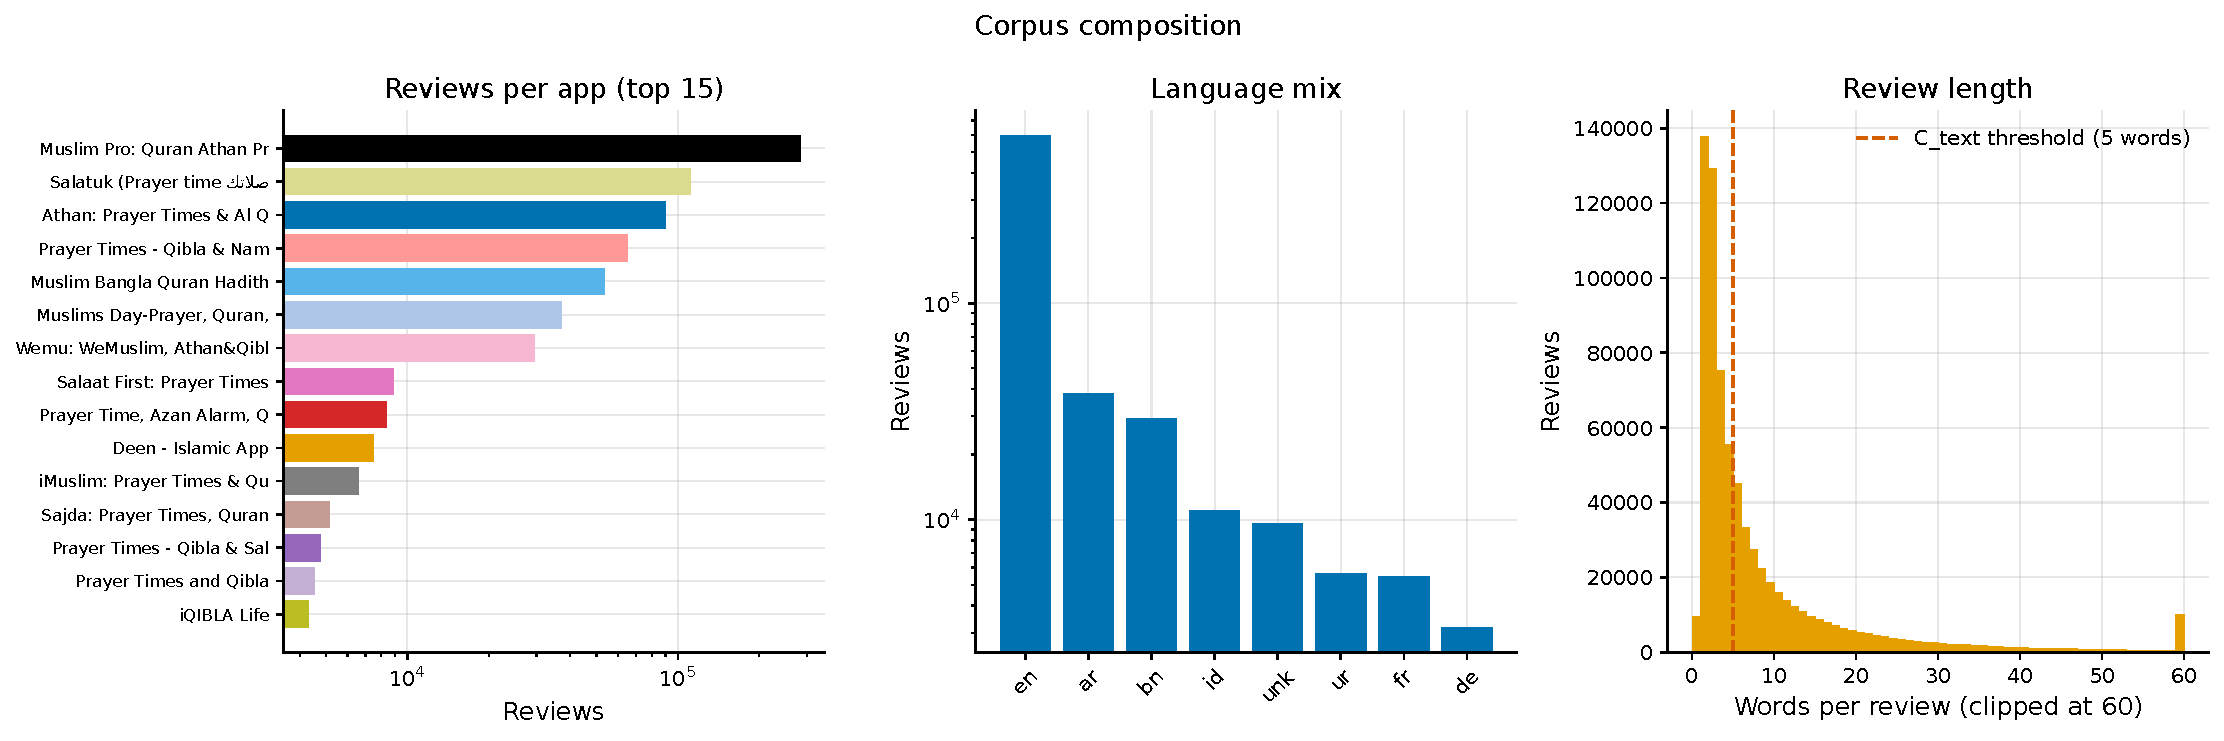
\includegraphics[width=\linewidth]{fig01_corpus_composition}
  \caption{Corpus composition: review volume for the 15 largest applications, language mix, and review-length distribution.}
  \label{fig:corpus}
\end{figure}

\subsection{Language Filtering and Analysis Sub-corpora}
\label{sec:method-language}

Reviews were filtered to those carrying review text, yielding an analysed
sub-corpus of 324,687 reviews (\(C_{\mathrm{text}}\)). Language identification
was then applied using fastText; the English-language subset used for topic
modelling comprises 276,422 reviews (\(C_{\mathrm{en}}\)).

\subsection{Sentiment Classification}
\label{sec:method-sentiment}

Reviews were scored in two passes: a lexicon-based pass with VADER and a
transformer-based pass with a RoBERTa sentiment classifier. The RoBERTa label is
the one reported throughout the paper, and VADER is retained as a comparison
point rather than as a source of any reported result.

Two separate checks bear on that choice, and we keep them apart because they
establish different things. First, agreement between methods across all 324,687
texted reviews (Figure~\ref{fig:sentiment-agreement}): RoBERTa agrees with the
star-derived label at Cohen's \(\kappa = 0.466\), against 0.210 for VADER, and
the two classifiers agree with each other at 0.385. Star ratings are not ground
truth --- RQ2 is in part an argument that they are not
(\S\ref{sec:rq2}) --- but RoBERTa tracking them more than twice as closely as
VADER does is the empirical reason we report the transformer label.

Second, we hand-labelled a 500-document gold set into four categories
(Positive, Neutral, Negative, Mixed); on the 100 rows coded by both annotators,
raw agreement was 89.0\% and Krippendorff's \(\alpha = 0.824\). We state plainly
what this does and does not establish: it is an inter-annotator reliability
figure showing that people apply the scheme consistently, not a measurement of
classifier accuracy against those labels, which we did not compute. Sentiment
therefore enters this paper as a comparatively, rather than absolutely,
validated variable, and the claims resting most heavily on it --- the
bimodality of tracker sentiment (\S\ref{sec:rq1}) and the feature-level
negative-sentiment rates behind RQ6a --- should be read with that gap in mind.

\begin{figure}[t]
  \centering
  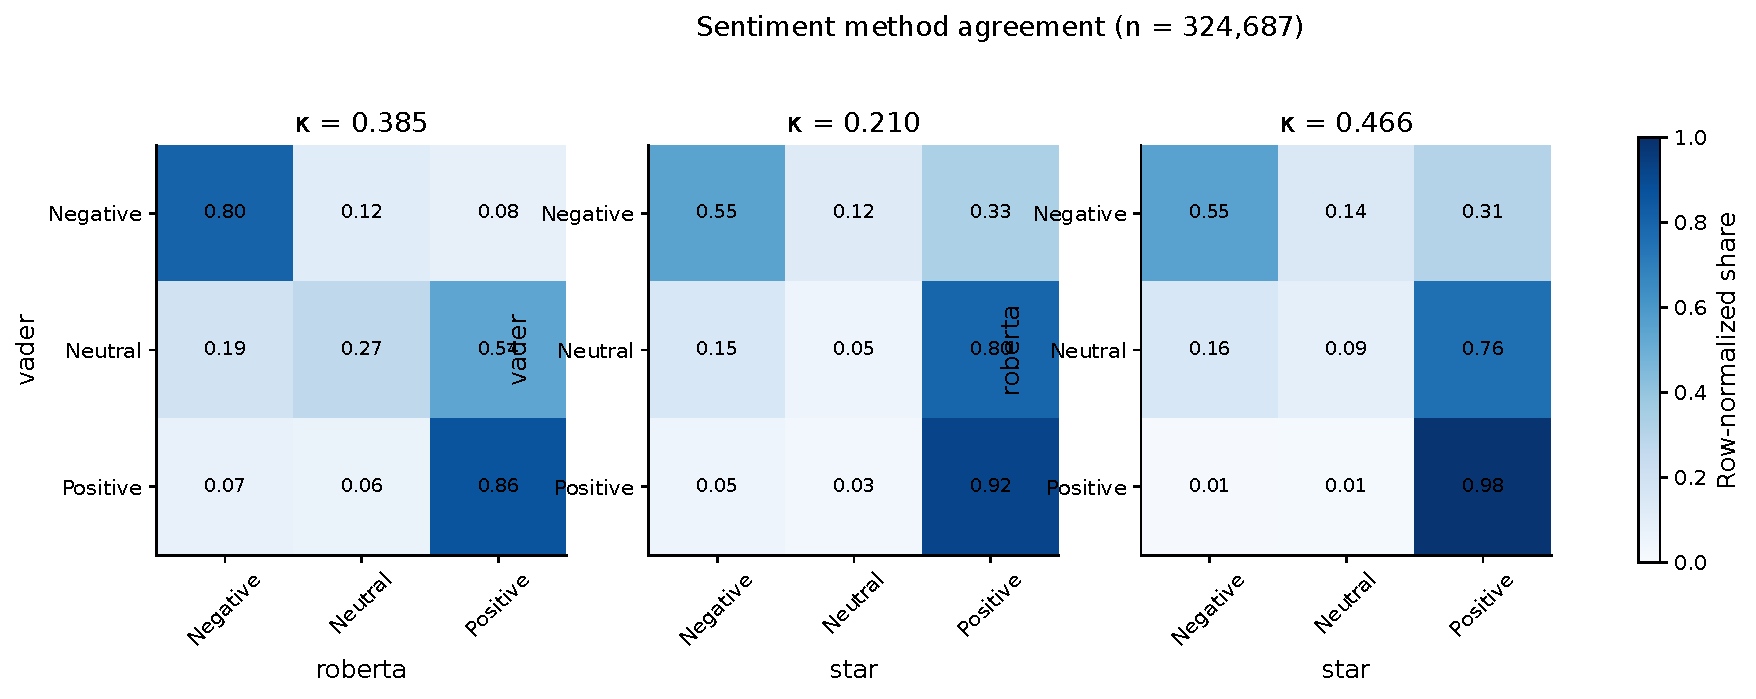
\includegraphics[width=\linewidth]{fig02_sentiment_agreement}
  \caption{Pairwise agreement between the three sentiment signals across the 324,687 texted reviews, row-normalised, with Cohen's \(\kappa\) per pair. RoBERTa tracks the star-derived label more closely (\(\kappa = 0.466\)) than VADER does (\(\kappa = 0.210\)).}
  \label{fig:sentiment-agreement}
\end{figure}

\subsection{Aspect-Based Sentiment Lexicon}
\label{sec:method-aspects}

We built a lexicon of 27 aspects covering the functional and experiential
surface of devotional apps (prayer-time accuracy, adhan reminders, Quran audio,
qibla direction, prayer tracking, advertising, monetisation, and others),
comprising 340 keywords and 106 regular-expression patterns applied at the
sentence level. Each sentence can carry zero, one, or multiple aspect tags.
Keyword and pattern counts vary widely across the 27 aspects, and since several
results below turn on how thinly a given aspect is defined, we release the
lexicon in full rather than summarising it: every aspect's exact keyword list
and patterns are in the artefact (\S\ref{sec:method-repro}), as are the aspect
groupings each research question composes from them.

\subsection{Affect Lexicon}
\label{sec:method-affect}

RQ1 additionally uses two small keyword lists, one guilt- and anxiety-related
and one motivation-related, to compare affective register inside and outside
tracker discourse. These differ from every other measurement in this paper in
one respect we state rather than leave to be found: they carry no gold sample
and no precision figure, because the 300-row aspect draw and the 500-document
sentiment set label aspects and valence, neither of which is the guilt/motivation
distinction. We release both lists with the analysis code, report the result
they produce as a lexical-frequency comparison rather than as a validated
measurement of guilt (\S\ref{sec:rq1}), and rest the construct claim on the
hand-coded passes instead.

\subsection{Devotional-Formula Filtering}
\label{sec:method-devotional-filtering}

After lexicon tagging, we removed aspect assignments whose triggering sentence
consists of devotional formulae rather than substantive feedback: 1,686 of the
192,874 aspect-tagged sentence pairs the lexicon produced (0.9\%), leaving
191,188. The unit is the (aspect, sentence) pair rather than the sentence, so a
sentence carrying two tags is counted twice. This step is necessary because general-purpose English feature
vocabulary misfires badly on devotional register. The clearest case is
\texttt{goal\_system}, which scored 0\% precision against its gold rows because
reviewers routinely close a review with phrases such as ``May Allah reward
you,'' which the lexicon's goal-related keywords match as if they described a
tracking feature. We treat this as a substantive finding rather than a cleaning
footnote: off-the-shelf sentiment and aspect tooling, built and validated on
general product review text, does not transfer cleanly to religious register,
and a devotional-formula filtering pass is necessary before aspect-level
analysis is trustworthy in this domain.

\subsection{Demand Mining}
\label{sec:method-demand}

We extracted five types of demand signal from review text via pattern
matching, each attached to the aspect(s) it co-occurs with: \emph{request}
(explicit asks for a feature), \emph{absence} (noting a feature is missing),
\emph{churn} (citing a missing feature as a reason for leaving or switching
apps), \emph{preference} (citing a feature as the reason for choosing an app),
and \emph{tenure} (citing a feature in the context of long-term use). Against a
200-row gold sample stratified 40 rows per type, overall precision was 91.5\%
(183/200): preference 100\%, tenure 100\%, churn 97.5\%, request 95\%, and
absence 65\%.

This figure carries a provenance caveat that we state plainly rather than
suppress. The gold sample was drawn and labelled from one run of the demand
extractor; an upstream threshold subsequently changed, the extractor was
re-run, and the regenerated output no longer matches the labelled sample
row-for-row (only 11 of the 200 labelled reviewIds recur in the current
extraction). The demand counts reported elsewhere in this paper come from the
current extraction, while the 91.5\% precision figure was measured on its
immediate predecessor. We report it as the best available estimate of demand-pattern
precision, with this provenance gap disclosed, rather than as a measurement of
the exact rows underlying every reported count.

\subsection{Promise Extraction}
\label{sec:method-promise}

To compare what an application promises against what it delivers, we extracted
claimed features from each app's Google Play store description and compared
them against a hand-built feature matrix (one row per app, one column per
aspect). Agreement between the two sources is weak: mean Cohen's
\(\kappa = 0.272\) across 20 features, with a maximum of 0.62 for women's
tracking and four features at \(\kappa = 0.00\) --- travel concession,
calendar integration, prayer times by location, and timely reminders. We
report this plainly rather than treat the two sources as interchangeable;
Figure~\ref{fig:promise-agreement} gives the per-feature breakdown, including
cases where the description misses a feature the matrix records and cases where
it overclaims one the matrix does not.

Those four zeros need reading carefully rather than at face value. In each
case one source records the feature in almost every application or in almost
none, so there is too little variance for \(\kappa\) to correct against, and
the coefficient collapses to zero despite high raw agreement: 96.2\% for timely
reminders (26 of 26 against 25 of 26) and 96.2\% for travel concession. Mean
raw agreement across the 20 features is 73.1\%. We report both summaries
because \(\kappa\) alone would understate how far the two sources actually
coincide on the features RQ6a and RQ3 depend on, while raw agreement alone
would flatter the features where the sources genuinely diverge.

\begin{figure}[t]
  \centering
  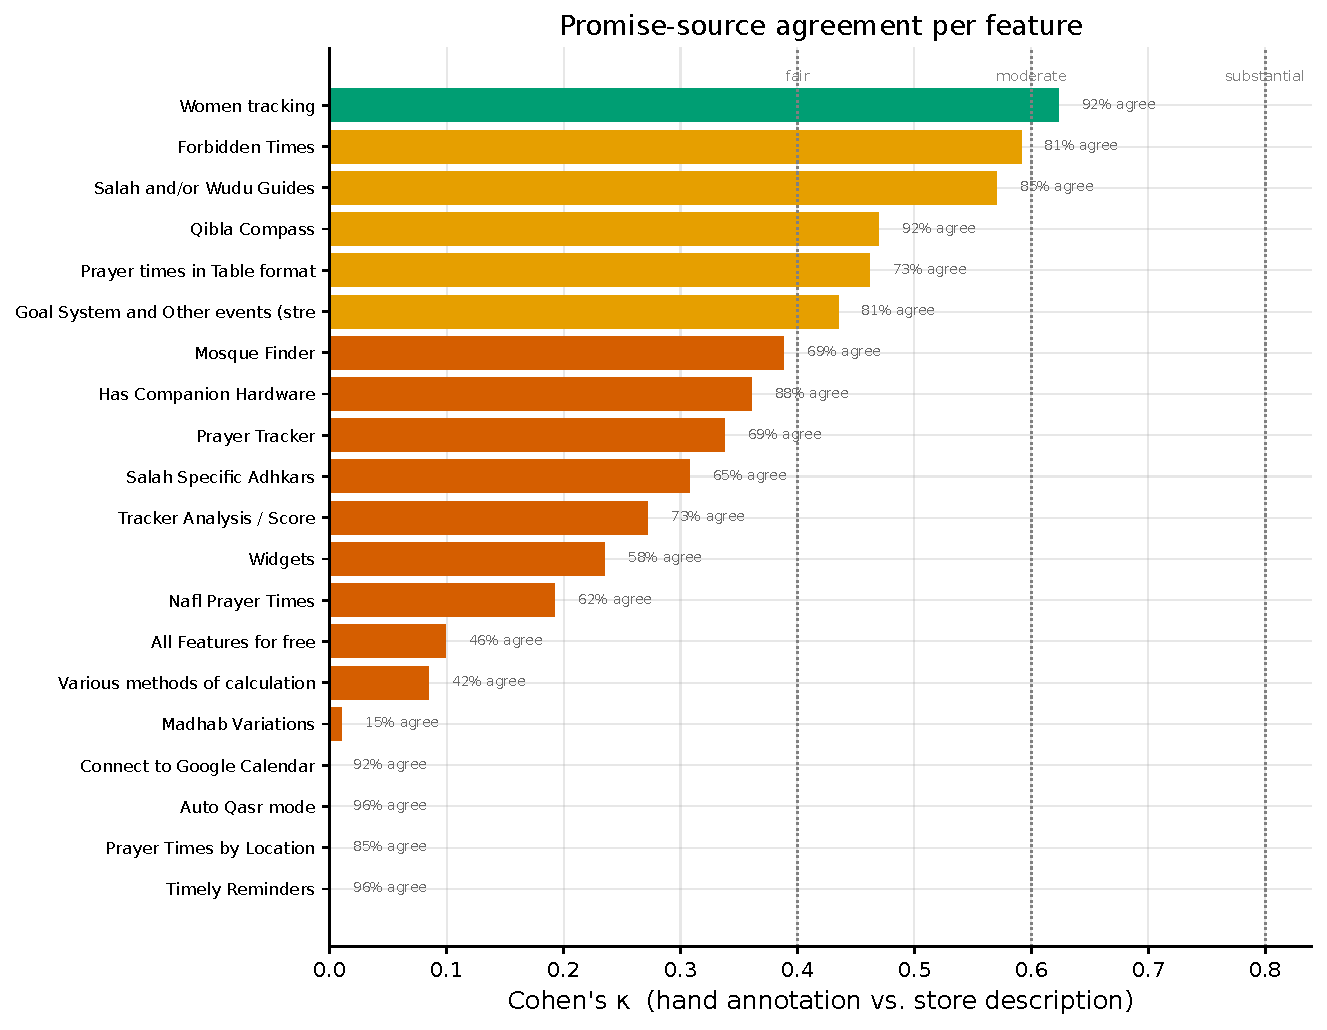
\includegraphics[width=\linewidth]{fig03_promise_source_agreement}
  \caption{Agreement between store-description promises and the hand-built feature matrix, by feature.}
  \label{fig:promise-agreement}
\end{figure}

\subsection{Topic Modelling}
\label{sec:method-topics}

We fit a BERTopic model over \(C_{\mathrm{en}}\) (276,422 documents) using a
seeded UMAP reduction and a stopword list extended with Islamic-domain terms
and application-name tokens, to prevent generic devotional vocabulary and
app-name mentions from dominating topic keywords. The ecosystem-level model
produced 40 topics plus an outlier bucket. Topic 0 is an undifferentiated
generic-praise cluster (168,054 documents, 61\% of modelled documents) and the
outlier bucket holds a further 62,745 (22.7\%); the remaining 39 topics, which
we label and report, cover approximately 45,600 documents (about 16\% of
\(C_{\mathrm{en}}\)). All 63 topics across the ecosystem model and three
targeted sub-models (described below) were labelled by hand across four
sheets, alongside each model's outlier bucket. We treat the topic model as characterising the interpretable minority
of the corpus, not the corpus as a whole, throughout the paper.

In addition to the ecosystem-level model, we fit three targeted sub-models on
aspect-restricted subsets to support RQ1 (tracker discourse), RQ4 (menstrual
and inclusion discourse), and RQ5 (feature-bloat discourse). Topic structure
under BERTopic is sensitive to the UMAP seed; we assessed this by refitting
each sub-model across five seeds fixed in advance (42--46), before inspecting
any result. The \texttt{rq1\_tracker} sub-model is stable (mean pairwise
Adjusted Rand Index 0.837); \texttt{rq5\_bloat} is not (6--11 topics across the
five seeds, mean pairwise ARI 0.452). Where we draw on \texttt{rq5\_bloat}, we
therefore claim the recurring themes rather than a specific partition into a
fixed number of topics.

\subsection{Statistical Models}
\label{sec:method-models}

We fit five models (M1--M5), one primary per research question for RQ1--RQ5:
M1 (RQ2, the competing costs of accuracy and interface complaints), M2 (RQ1,
sentiment by tracker tier), M3 (RQ4, inclusion), M4 (RQ5, feature bloat and
hardware), and M5 (RQ3, competitive edge features). RQ6 is answered
descriptively, by comparing promised features against the sentiment their
mentions record, and enters no inferential model. The primary specification for
each of the five is a review-level mixed-effects
model with a random intercept per application, which accounts for the fact
that reviews cluster within 26 apps of very different size and character. Where
a mixed model did not converge, we report a cluster-robust OLS fit on the same
data and specification as a sensitivity estimate, clustering standard errors on
application.

Coefficients from the primary specifications enter a single Benjamini--Hochberg
false-discovery-rate correction: 29 in total, of which 20 survive at
\(q < 0.05\). The family's composition needs stating precisely, because it
treats two kinds of refit differently. Cluster-robust refits are reported
alongside their primary counterparts and are not entered, since correcting a
robustness check against the test it checks would double-count the contrast.
The eight ordinal refits of M1's complaint terms \emph{are} entered, because
they change the outcome variable rather than only the error structure and so
constitute separate tests. We flag the asymmetry rather than leave it to be
inferred: it is a defensible line but not the only defensible one, and a reader
who would draw it elsewhere can recompute from the released coefficient
table.

Eleven terms cannot support inference, and we report all eleven rather than
silently dropping them; they divide into two kinds that sit differently with
respect to that denominator. Eight are mixed-model terms whose standard errors
are degenerate rather than merely large --- M2's two tracker-tier terms and six
from M4, with standard errors from \(4.1\times10^{2}\) to \(2.0\times10^{6}\)
and every one reporting \(p \approx 0.99999\). These eight do carry
\(q\)-values and are inside the 29, so read in isolation they resemble
``tested, not significant'' rather than ``failed to converge''; they account
for eight of the nine terms in the 29 that fail to survive correction, the
ninth being \texttt{madhab} in the ordinal specification, which we enter as a
primary term rather than a sensitivity refit and which returns a small,
imprecise estimate that reverses sign against M1 (\S\ref{sec:rq2}); we rest no
directional claim on it. The other three ---
M3's \texttt{women\_feature\_score\_diff}, M5's \texttt{has\_mosque\_finder},
and one M5 demand term --- return neither a standard error nor a \(p\)-value,
so they are outside the 29 rather than inside it, and no correction applies to
them at all. We
attribute the non-convergence to a structural cause: a random intercept per app,
fitted over only 26 apps, cannot be identified separately from an app-level
predictor in the same model. Throughout, we cite null results only from a model
that converged, and never describe one of these eleven as evidence of no effect.

\subsection{Measurement Quality}
\label{sec:method-measurement}

Because several of the paper's claims rest on aspect tags, we report their
precision directly rather than assuming lexicon output equals ground truth.
Against a 300-row gold sample, of which 192 rows still match under the current
lexicon configuration, unweighted aspect precision is 69.3\% and
corpus-volume-weighted precision is 84.4\% (95\% CI [79.7, 88.9]). The gold set
was originally labelled against an earlier, broader configuration including a
zero-shot backstop; every subsequent lexicon change has only removed matches,
never added them, so the 192 surviving rows are an unbiased subset of the
original 300 rather than a re-labelling exercise. Two aspects,
\texttt{calendar\_sync} and \texttt{goal\_system}, have no surviving gold rows
(together 0.2\% of aspect-tagged volume) and are excluded from the weighted
figure.

The weighted figure is driven by high-volume aspects and conceals substantial
variation. The 300-row gold draw sampled all 27 aspects at 11 rows each.
Table~\ref{tab:aspect-precision} reports precision for the 25 whose rows
survive the current lexicon configuration; \texttt{calendar\_sync} and
\texttt{goal\_system} lost all of theirs to lexicon narrowing. The 25 account
for all 192 surviving rows and for the weighted figure above. Seven of them
fall below 50\%, with gold samples as small as one or two rows. We report this
in full because several of these are load-bearing for individual research
questions: every aspect-level count drawn from one of the seven is reported
elsewhere as a precision-adjusted estimate with its interval, never as a bare
tagger count. Seventeen aspects sit at or above 64\% precision, and these
supply almost all model input, with two exceptions we flag rather than bury.
\texttt{madhab}, at 60\%, enters M1, and its coefficient is also the one M1
term that reverses sign under the ordinal robustness check, so we rest no
directional claim on it (\S\ref{sec:rq2}). And the mosque-finder contrast in
RQ3 is fit on the subset of reviews the \texttt{mosque\_finder} tagger selects,
which runs at 27\%; because the resulting noise falls on both arms of that
comparison rather than one, we read the direction of the gap and not its
magnitude, and say so at the point of use (\S\ref{sec:rq3}). No other model
term is drawn from an aspect below 50\% precision.

\begin{table*}[t]
  \centering
  \small
  \caption{Aspect-tagging precision against gold-standard rows, by aspect, for the 25 aspects whose gold rows survive the current lexicon configuration. Bold rows fall below 50\% precision; any count for these is reported elsewhere only as a precision-adjusted estimate with its interval. Gold samples are small, so the intervals are wide and we report them rather than the point estimate alone.}
  \label{tab:aspect-precision}
  \begin{tabular}{lrrrll}
    \toprule
    Aspect & Corpus \(n\) & Gold \(n\) & Precision & 95\% CI & Adjusted estimate \\
    \midrule
    reminders\_adhan        & 30{,}069 & 7  & 100\% & [65, 100] & \\
    quran\_audio            & 24{,}964 & 6  & 100\% & [61, 100] & \\
    prayer\_times\_accuracy & 21{,}941 & 11 & 73\%  & [43, 90]  & \\
    ads\_intrusive          & 17{,}845 & 11 & 100\% & [74, 100] & \\
    ui\_design              & 15{,}720 & 11 & 73\%  & [43, 90]  & \\
    monetization            & 13{,}914 & 11 & 82\%  & [52, 95]  & \\
    adhkar                  & 9{,}280  & 3  & 100\% & [44, 100] & \\
    qibla                   & 8{,}526  & 11 & 82\%  & [52, 95]  & \\
    stability\_bugs         & 7{,}665  & 11 & 64\%  & [35, 85]  & \\
    privacy\_data           & 7{,}471  & 10 & 90\%  & [60, 98]  & \\
    prayer\_tracker         & 6{,}009  & 9  & 78\%  & [45, 94]  & \\
    complexity\_bloat       & 5{,}389  & 9  & 67\%  & [35, 88]  & \\
    widgets                 & 4{,}755  & 11 & 100\% & [74, 100] & \\
    spiritual\_affect       & 3{,}395  & 2  & 100\% & [34, 100] & \\
    \textbf{mosque\_finder}      & 3{,}043 & 11 & \textbf{27\%} & [10, 57] & \(\approx\)830 [297, 1{,}721] \\
    \textbf{companion\_hardware} & 2{,}512 & 5  & \textbf{40\%} & [12, 77] & \(\approx\)1{,}005 [295, 1{,}932] \\
    \textbf{women\_period}       & 2{,}194 & 10 & \textbf{20\%} & [6, 51]  & \(\approx\)439 [124, 1{,}119] \\
    \textbf{forbidden\_times}    & 1{,}534 & 10 & \textbf{10\%} & [2, 40]  & \(\approx\)153 [27, 620] \\
    \textbf{table\_format}       & 1{,}483 & 9  & \textbf{44\%} & [19, 73] & \(\approx\)659 [280, 1{,}088] \\
    nafl\_times             & 963      & 5  & 100\% & [57, 100] & \\
    calc\_method            & 639      & 10 & 90\%  & [60, 98]  & \\
    \textbf{qasr\_travel}        & 637      & 2  & \textbf{0\%}  & [0, 66]  & do not report volume \\
    madhab                  & 491      & 5  & 60\%  & [23, 88]  & \\
    guides                  & 202      & 1  & 100\% & [21, 100] & \\
    \textbf{tracker\_score}      & 101      & 1  & \textbf{0\%}  & [0, 79]  & 1 gold row, uninformative \\
    \midrule
    Total                   & 190{,}742 & 192 & & & \\
    \bottomrule
  \end{tabular}
\end{table*}

Gold-sample size per aspect ranges from one to eleven rows, so these intervals
are wide; we treat the width as honest uncertainty rather than a reason to
report the point estimate alone. We also measured a zero-shot classification
backstop intended to supplement the lexicon, and dropped it after it scored
11.5\% precision on 300 hand-labelled sentences; we report this discarded
component as evidence of calibration during development rather than omit it.

\subsection{Research Ethics and Data Handling}
\label{sec:method-ethics}

The corpus is public store review text. No user was recruited, contacted, or
observed, and no account-linked or private data was accessed, so the study
involved no human participants and was not submitted for human-subjects
review. We none the less treat it as
data about people: the reviews concern religious observance, and some disclose
menstruation, illness, or lapses in practice, which a reviewer complaining about
a notification may not have understood themselves to be publishing. We
therefore report no reviewer names or identifiers, attribute quotations only to
an application and a star rating, and choose quotations carrying no incidental
personal detail. We quote verbatim rather than paraphrase, since altering
wording in a study whose claim concerns devotional register would misrepresent
the evidence, and we accept the residual risk that a short quoted string can be
matched back through store search. Two of our quotations disclose menstruation, the category we name above as
most sensitive. We judged the disclosure necessary: RQ4's claim is that users
voice this need explicitly, and paraphrase would convert direct evidence into
our own assertion of it. We chose the shortest instances that carry the point,
neither names an author, and both are already public and searchable. The
artefact releases derived data rather than redistributable raw review text
(\S\ref{sec:method-repro}). We name
applications throughout, including in criticism: they are public commercial
products, and the argument cannot be made without saying which application did
what. Where we name one in connection with a specific controversy rather than
an ecosystem pattern, we confine the claim to that episode
(\S\ref{sec:limitations}).

\subsection{Use of AI Assistance}
\label{sec:method-ai}

All analysis software for this study was written with the assistance of Claude
Code, Anthropic's command-line coding agent, driven interactively by the
authors. We disclose this because the assistance was substantive in the conduct
of the research rather than confined to preparing the manuscript. Three
boundaries bound what it can threaten. First, no generative model produced,
imputed, translated, or altered any review text, any label used as data, or any
reported statistic; every number here is the output of code executed over the
scraped corpus. Second, the design is the authors' own: the six research
questions were specified in a written analysis plan committed to version
control before the analysis was run, the aspect lexicon and the coding frame
were hand-built, and every gold-standard label was assigned by a human
annotator without model assistance. Third, the authors read, executed, and are
responsible for all code.

Assistant-written code can carry defects a human author would not introduce,
and we do not claim otherwise; our safeguards are the ones already reported ---
per-stage precision measured against hand-labelled gold sets, a component those
checks rejected at 11.5\% precision, the seed-stability pass, and the
byte-identical re-run below. One such defect was found and fixed during
analysis: the three sub-models shared a hardcoded output path and overwrote the
ecosystem topic sheet on each run. The sheet was rebuilt from the saved model
and stored assignments without refitting, and no reported statistic depended on
it. Confidence in the pipeline should rest on the checks that catch such
faults, not on an assumption that none occurred.

\subsection{Reproducibility}
\label{sec:method-repro}

The analysis reported in this paper was run on 2026-09-03 at commit
\texttt{5da2db7}. We subsequently re-ran the modelling stage from a clean tree
at the same commit and obtained byte-identical output, confirming
reproducibility of the reported coefficients. All stochastic components are
seeded: the UMAP reduction underlying topic modelling is seeded, and the five
seeds used for the topic-stability check (42--46) were fixed in advance of
inspecting any result, so the seed set could not be adjusted after the fact to
favour a particular outcome. A run manifest recording commit, hardware, batch
size, and library versions for every reported figure accompanies the research
artefact.

\paragraph{Data and code availability.} We release the full pipeline, the
aspect lexicon, the feature matrix, every hand-labelled gold and topic sheet,
the model output, and the run manifest, at a URL supplied on acceptance and
withheld here for anonymous review. Derived data sufficient to recompute every
table and figure is included. Two things are not: the raw review corpus, which
the store's terms do not permit us to redistribute and which carries the
re-identification risk noted in \S\ref{sec:method-ethics}, and the fitted model
binaries, which are large and reproducible from the seeded pipeline. The gold
sheets we do release carry the review text their labels apply to, since a
precision figure cannot be checked without it; that is a few hundred rows drawn
for verification rather than the corpus, and we judge the disclosure
proportionate on the same reasoning that governs quotation above. The
collection script and application list are included, so the corpus can be
re-gathered, though store histories change and an exact reconstruction of our
snapshot is not possible.

% results_rq1

\section{RQ1: Gamification}
\label{sec:rq1}

A recurring claim in the self-tracking literature is that gamified
mechanics --- streaks, scores, badges --- induce anxiety and guilt in users who
fail to keep them up. Prayer trackers add a streak or a completion score to the
five daily prayers, so RQ1 asks whether this tension appears in devotional
tracking specifically. It does not, in the form the literature predicts.
Gamifying a prayer tracker neither helps nor harms sentiment, and guilt
language is \emph{rarer} inside tracker discourse than in the corpus at large.
What users resent is a record they cannot trust and a prompt that never
arrives. We present this as a reframing of the streak-anxiety hypothesis, not
merely a null result on it.

\subsection{Scope}

We define tracker discourse as the union of reviews carrying at least one of
three aspect tags --- \texttt{prayer\_tracker}, \texttt{tracker\_score},
\texttt{goal\_system} --- which yields 6,285 reviews across 25 of the 26
applications. The union is a definition rather than a measurement --- it is
declared as a three-element list in the released analysis code, and the tags it
names are keyword-defined in the released lexicon --- so what it needs is not
validation but a statement of what it contains. That composition is uneven.
At review level, \texttt{prayer\_tracker}, at 78\% precision, accounts for
5,907 of the 6,285; 378 reviews (6.0\% of the set) carry only
\texttt{tracker\_score} or \texttt{goal\_system}, both of which score 0\%
against their gold rows, the latter being the devotional-formula failure
described in \S\ref{sec:method-devotional-filtering}. These are review counts,
not the tagged-sentence counts in Table~\ref{tab:aspect-precision}, which are
not subtractable from them. The disparity is visible in the
definitions themselves: \texttt{prayer\_tracker} carries 13 keywords and 4
regular-expression patterns, against 2 keywords and 4 patterns for
\texttt{tracker\_score} and 7 keywords and 2 patterns for
\texttt{goal\_system}, so the two weaker tags rest on markedly less lexical
evidence. Those two aspects enter after the devotional-formula filter has already removed
the sentence pattern causing the \texttt{goal\_system} misfire. We report the two analyses that run on the full
set --- the tier comparison and the dip test --- on that basis, noting that
noise at this share attenuates a distributional signal rather than
manufacturing one. The guilt test and both coding passes draw their own
samples from within the set and do not depend on its outer boundary.

\subsection{No Sentiment Difference by Tracker Tier}

We compared sentiment across three tiers of tracking mechanic: no tracker,
a plain tracker, and a tracker combined with a numeric completion score. The
primary mixed-effects specification (M2) did not converge on this contrast ---
its two tier terms return estimates of 13.66 and 13.87 with standard errors of
\(2.0\times10^{6}\) and \(1.3\times10^{6}\) and \(p \approx 0.99999\) --- so we
report the tier comparison from the cluster-robust OLS sensitivity fit, which
did converge. Against no tracker, a plain tracker gives \(\beta = -0.087\)
(95\% CI \([-0.332, 0.158]\), \(p = 0.488\)) and a tracker with a numeric score
gives \(\beta = -0.134\) (\([-0.415, 0.147]\), \(p = 0.349\)), clustered on 25
apps (\(n = 6{,}285\)). Both intervals sit comfortably across zero. Adding a
streak or a numeric score to a prayer tracker does not measurably move how
users feel about the application.

\subsection{Tracker Sentiment Is Bimodal}

A null on the mean, however, was never going to be the right test: the
love/hate tension the literature predicts is a claim about the \emph{shape} of
the sentiment distribution, not its centre. Hartigan's dip test on tracker
valence confirms this shape directly: \(D = 0.118\) (\(n = 6{,}285\)), and the
reported significance underflows machine precision, so we report \(p <
10^{-16}\) rather than \(p = 0\). Figure~\ref{fig:rq1-bimodal} shows the
distribution: tracker sentiment splits toward the two poles rather than
clustering in the middle, with users loving the tracker or resenting it and
comparatively little ambivalence between. This is why the qualitative coding
below, rather than the tier comparison, carries the substantive answer to RQ1.

\begin{figure}[t]
  \centering
  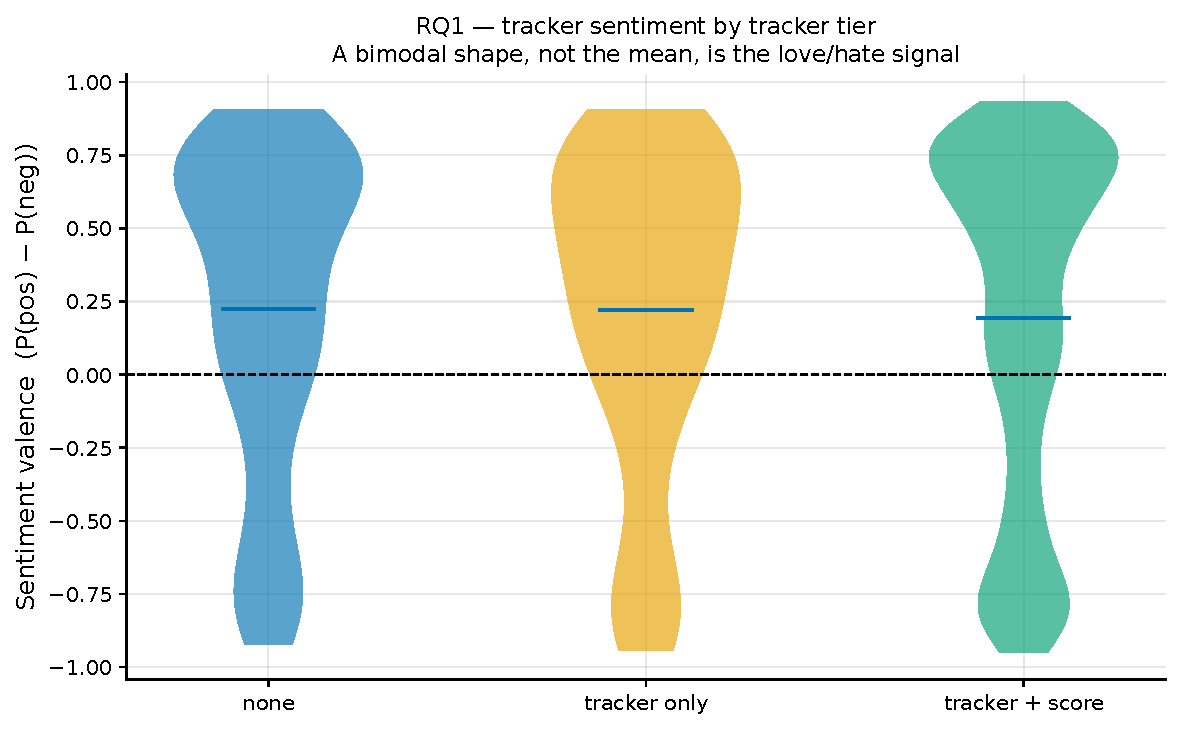
\includegraphics[width=\linewidth]{fig06_rq1_tracker_sentiment}
  \caption{Distribution of tracker-aspect sentiment valence, split by application tracker tier. Hartigan's dip on the pooled tracker set gives \(D = 0.118\), \(p < 10^{-16}\).}
  \label{fig:rq1-bimodal}
\end{figure}

\subsection{Guilt Is Rarer Inside Tracker Discourse, Not Commoner}

If streak anxiety were driving the negative pole of that split, guilt language
should be over-represented in tracker discourse relative to the rest of the
corpus. Two independent lines of evidence say it is not, and we keep them
apart because they establish different things.

The first is lexical. We match two keyword lists over review text, one of
guilt- and anxiety-related terms and one of motivation-related terms. Within
tracker reviews the ratio of guilt to motivation matches is 0.26, against 0.86
elsewhere in the corpus (Fisher exact OR \(= 0.283\),
\(p = 3.5\times10^{-11}\), \(q = 6.7\times10^{-11}\), \(n = 149\))
(Figure~\ref{fig:rq1-guilt}). We state the ceiling on this plainly: unlike the
aspect tagger and the demand patterns, these two lists were never validated
against hand-labelled rows, and their vocabulary is not construct-pure ---
\emph{helpful} and \emph{improve} are ordinary praise terms, and \emph{fail}
and \emph{stress} are ordinary defect terms. The result is therefore a fact
about the relative frequency of two lexicons, not a validated measurement of
guilt, and we release the lists with the code so the reader can judge them.

The second line is the hand coding below, where two independently drawn samples
were read and labelled by a person rather than matched by pattern. It points
the same way, and it is the evidence we rest the construct claim on. Where guilt-adjacent language does appear inside
tracker reviews, it is frequently folded into an otherwise positive,
motivational account rather than expressing distress:

\begin{quote}
\itshape ``I love the app. My everyday friend who reminds me to pray, and makes
sure that I feel guilty if I don't [\normalfont sweat-smile emoji\itshape] I
recommend to everyone who wants to start praying, or keep the habit in a
consistent manner!''
\end{quote}
\hspace*{1em}--- Athan: Prayer Times \& Al Quran, 5 stars

\noindent We mark the emoji rather than drop it, since it is the clearest
signal in the review itself that the guilt described here is light-hearted.

\begin{figure}[t]
  \centering
  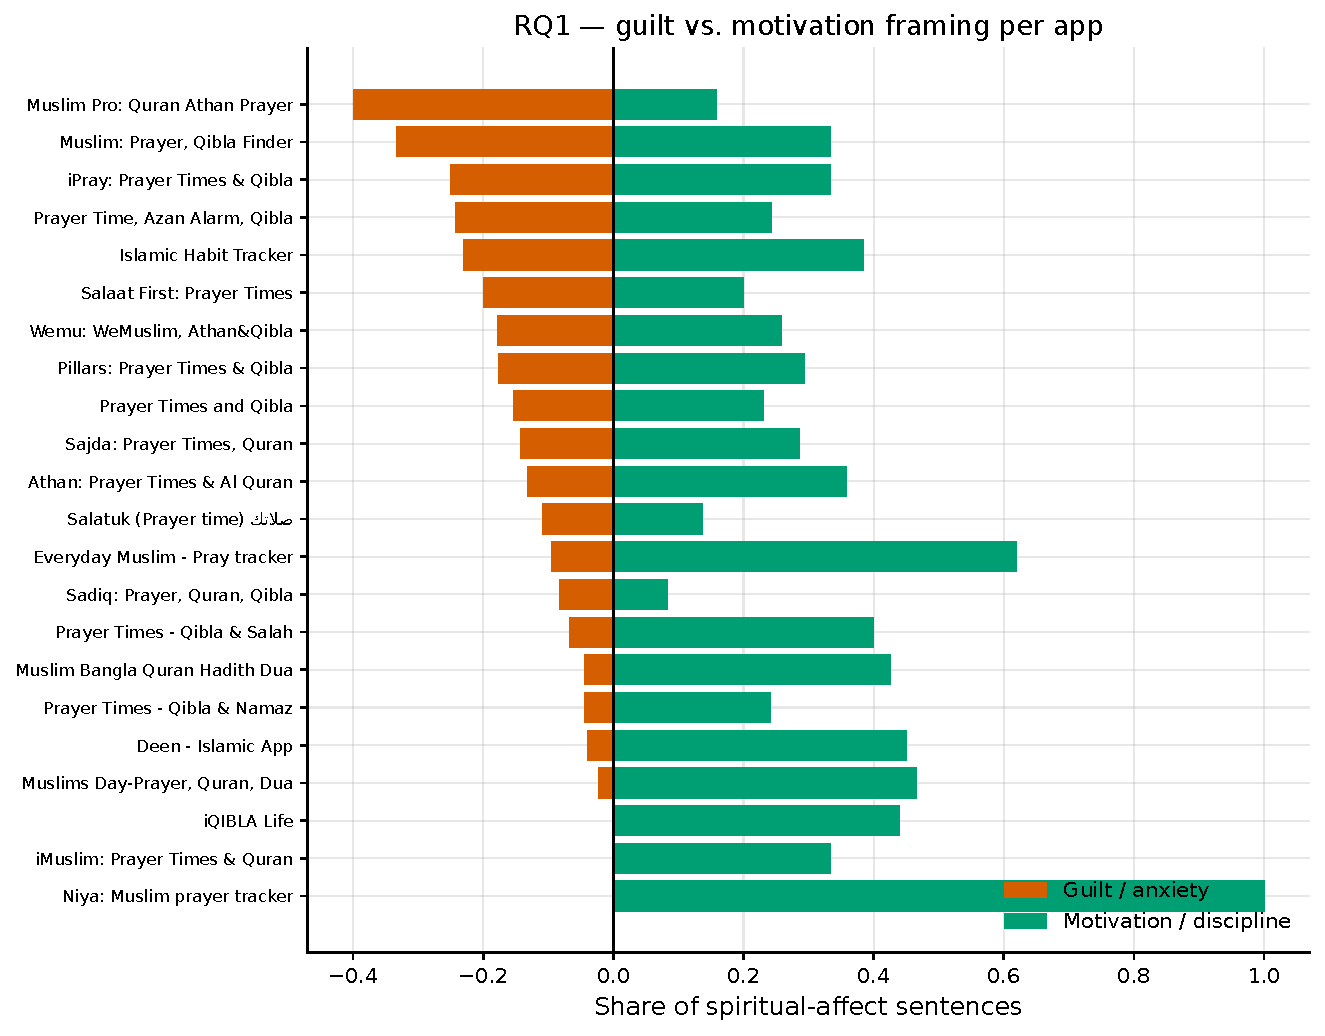
\includegraphics[width=\linewidth]{fig07_rq1_guilt_vs_motivation}
  \caption{Guilt- and motivation-coded affective language per application, as shares of that application's affect-coded reviews.}
  \label{fig:rq1-guilt}
\end{figure}

\subsection{Two Independent Coding Passes}
\label{sec:rq1-coding}

To characterise what tracker dissatisfaction is about, we coded two independent
samples of reviews expressing it --- this phrase rather than ``negative
reviews,'' since selection was by sentiment on the text rather than star
rating: 18 of the first sample's 50 carry 4--5 stars, so the set includes
otherwise-positive reviews built around one complaint. The first pass covered
50 reviews from a single application (\emph{Athan: Prayer Times \& Al Quran}),
selected before we identified that the selection rule's tie-break resolves
every three-valued sentiment tie in frame order, which here means app order;
the single-application sample is an artefact of that tie-break, not evidence
that one application dominates tracker complaints. The second pass drew 30
reviews stratified across the 22 other applications carrying codable tracker
dissatisfaction, no app contributing more than two, coded against the frame the
first pass produced.
Pass 1 yielded 33 open codes over 50 reviews (1 excluded, \(n = 49\)); pass 2
yielded 25 codes over 30 (2 excluded, \(n = 28\)) and required two new themes.
We report the passes side by side and never pool them, since their sampling
designs differ and a pooled percentage would silently re-weight the ecosystem
toward Athan (Table~\ref{tab:rq1-themes}).

\begin{table}[t]
  \centering
  \small
  \caption{Theme prevalence, coded independently in each pass. Never pooled.}
  \label{tab:rq1-themes}
  \begin{tabular}{lrr}
    \toprule
    Theme & Pass 1 (Athan, \(n{=}49\)) & Pass 2 (22 apps, \(n{=}28\)) \\
    \midrule
    C. Record can't be trusted        & 11 (22\%) & 6 (21\%) \\
    D. Normative mismatch             & 6 (12\%)  & 3 (11\%) \\
    E. Prompting failures             & 7 (14\%)  & \textbf{13 (46\%)} \\
    A. Redesign as regression         & 10 (20\%) & \textbf{0} \\
    B. Retroactive logging denied     & 5 (10\%)  & \textbf{0} \\
    F. Monetisation vs.\ religious purpose & 10 (20\%) & 1 (4\%) \\
    G. Record gated, not owned        & ---       & 3 (11\%)\(^\ast\) \\
    H. App overreaches into device    & ---       & 2 (7\%)\(^\ast\) \\
    \bottomrule
  \end{tabular}
  \\[2pt]
  {\footnotesize \(^\ast\)new theme, not present in the pass-1 frame}
\end{table}

Guilt or judgment is rare in both passes, and we give the two rates separately
rather than pooling them: 2 of the 49 coded complaints in the single-app pass
(4.1\%; \emph{tracker framing feels judgmental} and \emph{imposed goals replace
own tracking}) and 1 of the 28 in the cross-app pass (3.6\%; \emph{reminders
induce guilt}). A hypothesis this prominent in the self-tracking literature
surfacing at four percent or below in each of two independently drawn samples,
while the Fisher test above points the same way, is a robust null rather than
an underpowered one.

The two passes also demonstrate a general methodological hazard for app-store
review mining. Themes A, B, and F together account for 51\% of the single-app
pass's coded complaints but only 4\% of the cross-app pass's --- a concrete
case of single-app qualitative sampling manufacturing what looks like a
genre-level theme from what is, on a wider sample, a property of one
application's release.

\subsection{What Dissatisfaction Is Actually About}

Coding the cross-app sample against the shared frame surfaces a consistent
ordering, and it replicates across both independently drawn samples for two of
the three themes.

\textbf{Prompting failure is the dominant complaint ecosystem-wide (46\% of
the cross-app pass).} The tracker does not fail because logging is onerous;
it fails because the app never reliably prompts in the first place ---
location detection failing, adhan playback not firing, notifications lost,
calendars drifting out of sync:

\begin{quote}
\itshape ``the adhan is not working unless I open the app without logging out
of it till prayer time''
\end{quote}
\hspace*{1em}--- Pray Watch, 1 star

\textbf{Record trustworthiness replicates almost exactly across both samples}
(22\% in pass 1, 21\% in pass 2): users lose logged history, watch counts
regress, or find the tracker has silently disabled itself, often inside
reviews that otherwise praise the app:

\begin{quote}
\itshape ``I would give it a 5 star, but the prayers that I log on the
previous days or current day would sometimes disappear. Please fix this!''
\end{quote}
\hspace*{1em}--- Athan: Prayer Times \& Al Quran, 4 stars

\textbf{Normative mismatch is the smallest of the three replicating themes}
(\(\sim\)11\% in both passes) and is not the same construct as guilt. Where a
tracker review raises a genuinely normative objection, it is that the app
\emph{mis-models} religious practice, not that it makes the user feel
judged: menstrual exemption from prayer is unsupported, there is no support
for supererogatory (\emph{sunnah}) practice, and imposed goals displace the
user's own targets. We treat this distinction as the paper's contribution
here, not a restatement of the streak-anxiety story:

\begin{quote}
\itshape ``It's a really good app but I'm taking 1 star away cause I wish
there was some option for menstruating women cuz my overall score on prayer
tracker becomes really low when I can't pray for my period.''
\end{quote}
\hspace*{1em}--- Deen - Islamic App, 3 stars

\noindent Menstrual-exemption complaints of this kind appear independently in
\emph{both} coding passes, from different applications, and we return to them
as direct evidence for RQ4 (\S\ref{sec:rq4}).

\subsection{Themes A and B Are an Application-Specific Episode}

Two of the six original themes --- redesign as regression (20\% of pass 1) and
retroactive logging denied (10\%) --- vanish entirely in the cross-app pass.
Both concern a single redesign of the Athan tracker that broke an existing
logging workflow and removed retroactive logging. Because this pair accounted
for 30\% of the single-app sample's coded complaints, we report it as an
application-specific episode rather than folding it into any ecosystem-level
theme; conflating the two would overstate how much of tracker dissatisfaction
is about record integrity in general.

\subsection{Summary}

Adding a streak or a score does not move sentiment, and tracker sentiment is
bimodal, so a mean was never going to characterise it. Guilt language is
under-represented rather than over-represented inside tracker discourse, and
appears in 2 of 49 coded complaints in the single-app pass and 1 of 28 in the
cross-app pass. What tracker dissatisfaction is actually about, ecosystem-wide, is
the app failing to prompt reliably and failing to keep a trustworthy record;
where a normative objection surfaces, it concerns the app's model of worship
rather than pressure to perform.

% results_rq2

\section{RQ2: Accuracy Versus Interface}
\label{sec:rq2}

A second common framing in the review-mining and mobile-HCI literature treats
accuracy and interface polish as a trade-off users weigh against one another.
RQ2 asks whether devotional-app users punish inaccuracy more harshly than a
poor interface. As a class, they do not. That comparison, however, is the
wrong one to draw: the class-level average hides a severity gradient inside
accuracy itself, and the rating signal developers typically optimise against
conceals the worst of it.

\subsection{As Classes, Accuracy and Interface Cost the Same}

Using M1, a review-level mixed-effects model of star rating against complaint
aspect (\(n = 324{,}687\); all coefficients discussed in this section survive
Benjamini--Hochberg correction at \(q < 0.05\)), the accuracy family ---
prayer-time accuracy, qibla, madhab, and calculation method --- averages
\(-0.647\) stars, against \(-0.600\) for \texttt{ui\_design}. The gap is under
a twentieth of a star. The intuition that users punish a wrong qibla or prayer
time more harshly than a cluttered screen is not supported at the level of the
complaint class, and we do not claim accuracy wins as a class.

\subsection{The Class Average Conceals a Severity Gradient}

Table~\ref{tab:rq2-coefficients} and Figure~\ref{fig:rq2-coefficients} give the
full spread underlying that average. Accuracy is not one thing: prayer-time
accuracy alone costs \(-1.112\) stars (95\% CI \([-1.142, -1.083]\)), 1.85
times the interface penalty, with a confidence interval disjoint from
\texttt{ui\_design}'s. The family mean is pulled down by \texttt{madhab}
(\(-0.324\)) and \texttt{qibla} (\(-0.550\)), which are both rarer and milder
complaints. Getting the prayer time wrong is among the most costly failures in
the entire corpus; getting the madhab option wrong is among the least ---
and \texttt{madhab} additionally reverses sign in an ordinal robustness check
(\(\beta = +0.216\), \(p = 0.649\)), so no directional claim rests on it
either way.

\begin{quote}
\itshape ``this app is not accurate, prayers time are 1 hour ahead, please fix
it''
\end{quote}
\hspace*{1em}--- Athan: Prayer Times \& Al Quran, 1 star

\begin{table}[t]
  \centering
  \small
  \caption{M1 coefficients on star rating, all complaint aspects surviving BH-FDR at \(q < 0.05\) (\(n = 324{,}687\)).}
  \label{tab:rq2-coefficients}
  \begin{tabular}{lrr}
    \toprule
    Complaint & \(\beta\) & 95\% CI \\
    \midrule
    Intrusive ads            & \(-1.439\) & \([-1.460, -1.418]\) \\
    Prayer-time accuracy     & \(-1.112\) & \([-1.142, -1.083]\) \\
    Stability / bugs         & \(-0.938\) & \([-0.965, -0.910]\) \\
    Reminders / adhan        & \(-0.845\) & \([-0.868, -0.823]\) \\
    UI design                & \(-0.600\) & \([-0.664, -0.537]\) \\
    Calculation method       & \(-0.600\) & \([-0.769, -0.430]\) \\
    Qibla                    & \(-0.550\) & \([-0.594, -0.507]\) \\
    Madhab                   & \(-0.324\) & \([-0.526, -0.122]\) \\
    \bottomrule
  \end{tabular}
\end{table}

\begin{figure}[t]
  \centering
  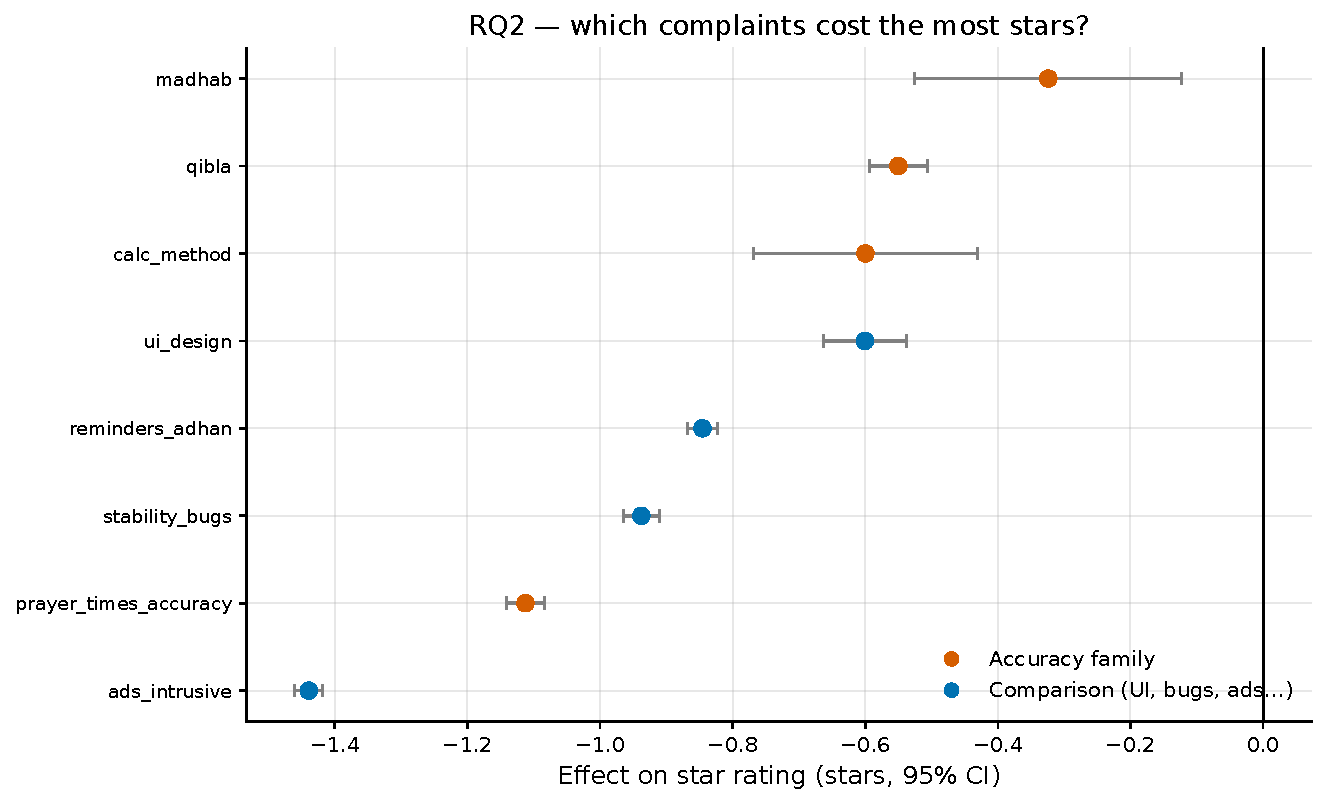
\includegraphics[width=\linewidth]{fig05_rq2_complaint_effects}
  \caption{M1 coefficients by complaint aspect, colour-coded by family. The spread within the accuracy family is visible directly in the error bars.}
  \label{fig:rq2-coefficients}
\end{figure}

\subsection{Qibla Failure Is Instability, Not Miscalculation}

The larger of the two qibla-related topics in our topic model (1,771 reviews)
is labelled around wrong direction, outweighing a second, smaller topic
(698) labelled around an inaccurate compass pointer. Reading the representative
reviews in the larger topic, the complaint is not that the app computes the
wrong bearing: users describe the compass returning a different bearing from
the same physical spot as the phone is rotated. We report this as a sensor and
calibration-handling problem rather than an error in the underlying qibla
computation, since the two failure modes call for different fixes.

\subsection{Star Ratings Hide Accuracy Defects}

The strongest result in RQ2 is methodological rather than substantive. Of
7,942 reviews carrying at least one negative accuracy-family complaint, 3,306
(41.6\%) awarded four or five stars, and 1,830 (23.0\%) awarded the maximum of
five; the full distribution runs 2,319 one-star, 914 two-star, 1,403
three-star, 1,476 four-star, and 1,830 five-star. Users report that the prayer
time or qibla direction is wrong and rate the application highly in the same
review.
Any prioritisation process that reads defect severity off the star
distribution --- which is to say, the signal most developers and app-store
ranking systems optimise against --- will under-weight accuracy defects by a
wide margin, because a substantial share of the reviews that name them never
produce a low rating.

\subsection{Advertising Costs More Than Any Accuracy Complaint}

One coefficient in Table~\ref{tab:rq2-coefficients} falls outside the
accuracy/interface contrast entirely and is worth flagging here: intrusive
advertising costs \(-1.439\) stars, above every accuracy-family term,
including prayer-time accuracy. We return to advertising as a recurring cost
across the bloat and gap analyses in \S\ref{sec:rq5} and \S\ref{sec:rq6}.

\subsection{Summary}

Accuracy and interface complaints are indistinguishable as classes, but that
comparison obscures more than it reveals. Prayer-time accuracy alone is a
severe, frequent failure whose cost is masked twice: once by averaging it with
milder accuracy complaints such as madhab and qibla, and again by arriving
inside four- and five-star reviews at a rate of 41.6\%. Star ratings are an
unsafe proxy for defect severity in this domain.

% results_rq3

\section{RQ3: Travel and Competitive Edge}
\label{sec:rq3}

A third framing common in mobile-app HCI research is that differentiating
features win and retain users --- that a distinctive capability such as a
mosque finder or a travel prayer-shortening (\emph{qasr}) mode confers a
competitive edge. RQ3 tests this against what users actually cite as reasons
for loyalty, and against the sentiment record of apps that ship these two
travel-oriented features. Neither supports the differentiation story: what
earns loyalty in this ecosystem is the reliability of core functions, not
travel support specifically.

\subsection{What Users Cite Is Not Travel Support}

Across 4,696 preference citations in the corpus --- reviews explicitly stating
why the user chose or kept an app, in the register of ``that's why I use
this'' or ``only app that'' --- the aspects named most are adhan reminders
(374), Quran audio (293), prayer-time accuracy (290), qibla (155), and adhkar
(152). Mosque finder does not appear in the top eight cited aspects, and qasr
does not appear at all. Preference-citation rates are close to identical
whether an app ships a mosque finder or not: 1.38\% of reviews for the 12 apps
that have one, against 1.24\% for the 14 that do not. Whatever earns loyalty
in this ecosystem, it is not the travel feature set.

\subsection{The Mosque-Finder Coefficient Runs the Wrong Way, and the Reason Matters}

A cluster-robust fit on reviews mentioning mosque finder gives
\(\beta = -0.137\) (\(p = 0.003\), 21 app clusters, \(n = 3{,}010\)): apps that
\emph{have} a mosque finder attract more negative mentions of it, not fewer
--- 27.0\% negative against 23.0\% in apps without the feature, with positive
mentions moving the other way (38.6\% against 43.6\%). Before reading anything
into that direction, we note that the \texttt{mosque\_finder} tagger runs at
27\% precision (95\% CI [10, 57]), so of the 3,010 mentions entering
this comparison, drawn from 3,043 tagged corpus-wide, roughly 830 are genuine
(interval [297, 1{,}721]);
we do not report either figure unqualified anywhere in this paper. The noise falls on both arms of the
comparison rather than one, so the \emph{direction} of the gap is more
trustworthy than its exact \emph{size}.

The direction should not be read as the feature harming apps that ship it. The
two groups of mentions are not comparable speech acts. Of the 14 applications
without a mosque finder, 11 draw any mention of one, and there mentions are
overwhelmingly \emph{requests} --- 243 demand signals across 9 apps --- which
phrased as ``please add nearby mosques'' read neutral-to-positive. Of the 12
that have the feature, 10 draw mentions, and there they are \emph{usage
reports}; a usage report of a feature that fails to work reads negative. The
21 applications drawing mentions at all are the clusters in the model above. A user can only complain about a feature
that exists to complain about. The gap therefore measures the difference
between wishing for a feature and using one, not the cost of having shipped
it.

This coefficient is also unstable across specifications, which we take as
further reason not to over-read its direction: the mixed-effects fit on the
same contrast returns \(+0.05\) with an undefined (NaN) standard error, and
so cannot arbitrate between the two estimates. We treat the cluster-robust
estimate as the more trustworthy of the two, but rest no directional claim
about competitive advantage on a coefficient that reverses sign between
specifications, one of which failed to produce an error estimate at all.

\subsection{Qasr Travel Concession: Demand Evidence, Not a Causal Test}

Exactly one application of the 26, \emph{Muslim Bangla Quran Hadith Dua},
implements qasr (the Islamic travel concession shortening obligatory
prayers). With \(N = 1\), there is no between-app comparison available for
this feature, and we treat the qasr result as demand evidence rather than as
a test of any causal claim. Demand is real, if modest: 21 signals in total
--- 10 requests, 5 preference citations, 3 explicit statements of absence,
and 3 churn statements --- of which 20 come from 5 of the 25 apps that lack
the feature. The requests are specific and practical:

\begin{quote}
\itshape ``My second suggestion is that prayer times automatically adjust when
I'm traveling because man forgets and my prayers be off.''
\end{quote}
\hspace*{1em}--- Muslim Pro: Quran Athan Prayer, 4 stars

\begin{quote}
\itshape ``please add namaz qasar for all 5 prayers \ldots\ while anyone is out
of city or in traveling''
\end{quote}
\hspace*{1em}--- Prayer Times - Qibla \& Namaz, 5 stars

\begin{quote}
\itshape ``I wish it was installed prior my hajj trip''
\end{quote}
\hspace*{1em}--- Athan: Prayer Times \& Al Quran, 5 stars

A measurement caveat applies to the broader \texttt{qasr\_travel} aspect tag,
distinct from these 21 hand-read demand signals. That tag matches 637
mentions across 18 apps and runs 76.7\% positive against only 7.1\% negative
--- implausible for a capability 25 of the 26 apps lack --- and scored 0 of 2
on its gold-standard rows. Only 3.3\% of its matches are demand signals. The
lexicon is evidently catching travel and pilgrimage discourse in general
(hajj, umrah, journeys) rather than qasr functionality specifically. We
therefore never report 637 as a measure of qasr discussion volume, and rest
the qasr argument entirely on the 21 demand signals, which were read directly
rather than inferred from the lexicon match.

\subsection{Dominant Travel Failure Mode}

Where travel-related failures do appear, the recurring pattern is that prayer
times fail to adjust automatically when a user's location changes, and the
user discovers this only after acting on a stale time:

\begin{quote}
\itshape ``The only thing that I don't like about this app is it doesn't seem
to automatically change your location when traveling until you physically
refresh the prayer times page. Unfortunately today I accidentally broke my
fast 1 minute early b/c the location was still set to an area almost 1 hour
away, pls fix this inshaAllah.''
\end{quote}
\hspace*{1em}--- Athan: Prayer Times \& Al Quran, 4 stars

\subsection{Summary}

Neither travel-oriented feature confers a competitive edge. Mosque finder is
not among the top eight aspects users cite for loyalty, and its sentiment gap
reflects the difference between requesting and using a feature, not a cost of
shipping it. Qasr has essentially no market presence and rests on demand
evidence alone. What users do cite --- adhan reminders, Quran audio,
prayer-time accuracy --- points back to core functions, and those are
themselves among RQ6's most-broken promises (\S\ref{sec:rq6}). Competitive
advantage here looks like doing the basics reliably.

% results_rq4

\section{RQ4: Bio-Spiritual Inclusion}
\label{sec:rq4}

Islamic law exempts menstruating women from the obligation to pray, and a
prayer tracker that does not represent this exemption misrepresents the
practice it claims to track. RQ4 asks how well the ecosystem serves that need.
Designers do not disagree about how to handle it: almost no one has built it,
the few implementations that exist are not trusted by their own users, and
demand is voiced explicitly and repeatedly across nearly the whole ecosystem.
Inclusion here is an unmet need, not a contested design question.

\subsection{Scarcity Is the Finding}

The \texttt{women\_period} tagger produces 2,194 aspect-tagged sentences,
resolving to 2,182 distinct reviews across the 24 of 26 applications carrying
any (Figure~\ref{fig:rq4-women-aspect}). Its precision is only 20\% (95\% CI
[6, 51]), so we report an adjusted estimate of roughly 439 genuine mentions
(interval [124, 1{,}119]), still spread across nearly the entire ecosystem.
RQ6's promise-and-delivery analysis works from a narrower basis of 1,981
reviews, which is where the sentiment rates below come from; we name all three
units rather than let one stand in for another. Only three applications ---
Athan, Islamic Habit Tracker, and Pillars --- ship any menstrual handling at
all. The rest of this section rests on demand signals and this three-app
scarcity, neither of which depends on the tagger's precision.

\begin{figure}[t]
  \centering
  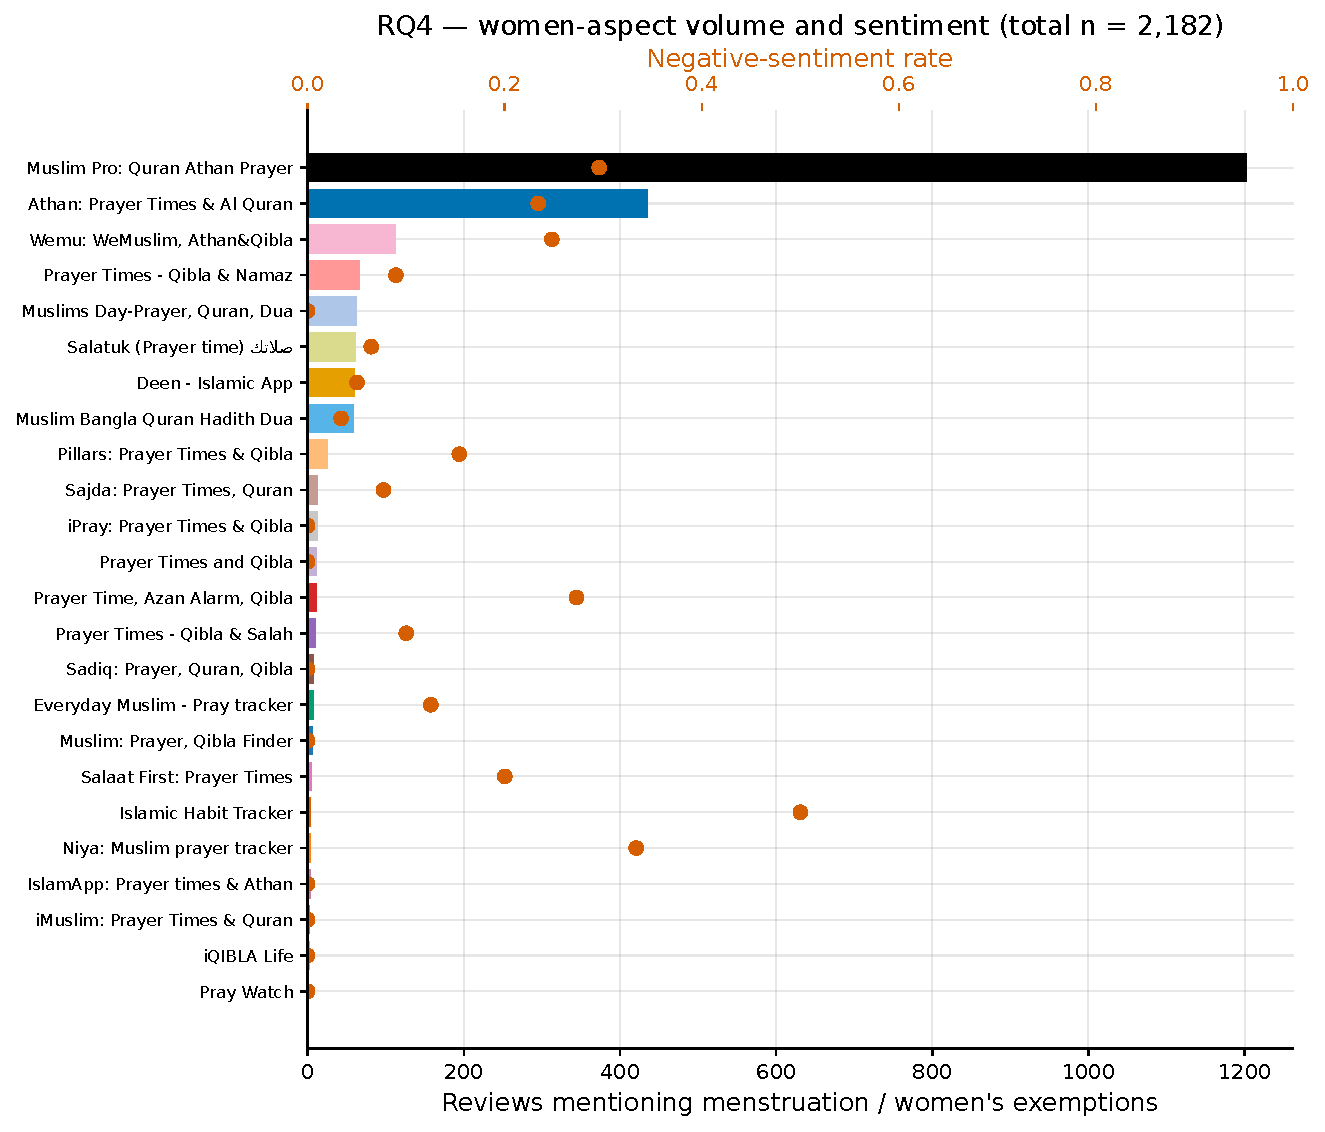
\includegraphics[width=\linewidth]{fig09_rq4_women_aspect}
  \caption{Reviews mentioning menstruation or prayer exemptions, by application, with negative-sentiment rate. The three applications shipping menstrual handling are named in the text.}
  \label{fig:rq4-women-aspect}
\end{figure}

\subsection{Demand Is Explicit, and Concentrated Where the Feature Is Absent}

Demand-pattern extraction, validated at 91.5\% precision
(\S\ref{sec:method-demand}), is the firm ground here. The 272 demand signals
tagged to \texttt{women\_period} break down into 161 explicit requests, 51
preference citations, 36 churn statements, 21 statements of absence, and 3
tenure citations; 216 come from the 16 applications that both lack the feature
and draw any demand, out of the 23 lacking it. These are signal counts, and one
review can carry several: the same demand resolves to 206 distinct reviews,
the unit RQ6b's unmet-need index uses (\S\ref{sec:rq6}). The register is
direct rather than incidental:

\begin{quote}
\itshape ``a feature for sisters who are on their monthlies would be nice so
they can keep track''
\end{quote}
\hspace*{1em}--- Muslim Pro: Quran Athan Prayer, 4 stars

\subsection{Having the Feature Does Not Improve Sentiment}

If the gap were purely one of coverage, the three applications shipping
menstrual handling should show better sentiment on the topic. They do not:
mentions run 26.3\% negative in those three against 26.0\% in the 21 lacking it
that draw any mention. Shipping the feature is not associated with users being
happier about it, which points at the quality of existing implementations
rather than availability alone:

\begin{quote}
\itshape ``The only complaint I have is: when I turn on menstrual mode it
doesn't turn off the prayers as it promises to do. Please fix it''
\end{quote}
\hspace*{1em}--- Athan: Prayer Times \& Al Quran, 4 stars

\noindent The RQ1 coding corroborates this independently: \emph{menstrual mode
unreliable} appears three times in the single-app pass, and \emph{menstrual
exemption absent} once in the cross-app pass, from a different application
(\S\ref{sec:rq1-coding}). Across two independently drawn samples, this is rare
first-hand evidence that the failure is one of execution as well as coverage.

\subsection{The Between-App Comparison Is Not Estimable}

With three applications on the treated side, no causal or comparative claim
about star rating is possible, and the data show why. The review-weighted
difference in mean star rating is \(+0.085\) (95\% CI \([+0.074, +0.096]\),
computed from the two review pools rather than from M3, whose
\texttt{women\_feature\_score\_diff} term returns neither a standard error nor a
\(p\)-value): apps with the feature average 4.476 stars against 4.391 without
(46,741 reviews across 3 treated apps, 277,946 across 23 untreated).
Averaging first by app and then across apps reverses the sign to \(-0.236\)
(4.135 against 4.371). Both are arithmetically correct and answer different
questions: Athan alone contributes 44,954 of the treated reviews, so the
review-weighted figure is close to one application's rating, while the
unweighted one is pulled down by Islamic Habit Tracker, the corpus's
lowest-rated application. We report \(+0.085\) and label it not estimable
rather than null. A difference reversing direction under a change of
aggregation, on three treated applications, is the clearest demonstration that
\(N = 3\) cannot answer this question.

\subsection{The Topic Model Cannot Add Resolution}

A sub-model fit on women's-health and privacy discourse does not separate
cleanly: after hand-labelling, five of its ten topics carry an identical label
describing one application's data being sold to the US military and a sixth is
a near-duplicate, so six of ten topics sit on a single theme holding 58\% of
the sub-model's non-outlier documents (4,788 of 8,285). One application's
data-handling controversy dominates the subset to the point that the sub-model
cannot further resolve menstrual-handling discourse. We report recurring themes
rather than treat the partition as ten findings, and return to the episode in
\S\ref{sec:limitations}.


% results_rq5

\section{RQ5: Feature Bloat and Companion Hardware}
\label{sec:rq5}

A fourth framing holds that adding features drives complaints about clutter and
complexity --- that a leaner app is a more satisfying one. We tested this on a
pre-specified hypothesis and test, before running the full corpus
(\S\ref{sec:rq5-provenance}). It fails in both directions: feature count does
not predict bloat complaints, and if anything the relationship runs backward.
What users mean by ``bloat'' is a property of the interface, not a count of
capabilities.

\subsection{Feature Count Does Not Predict Bloat Complaints}

The primary mixed-effects specification (M4) did not converge on its
\texttt{feature\_count} term (\(\beta = -0.004\), SE \(743.8\),
\(p \approx 0.99999\)), so we report this null from the cluster-robust
sensitivity fit, which did: the interaction
\texttt{complaint\_complexity\_bloat} \(\times\) \texttt{feature\_count} gives
\(\beta = -0.000487\) (95\% CI \([-0.00136, 0.00038]\), \(p = 0.272\)),
clustered on 26 apps. Adding features does not make users more likely to call
an app bloated. Nor is the null an artefact of a few large, well-known apps
absorbing the variance: feature count correlates only weakly with install count
across the 26 (Spearman \(\rho = 0.244\)).

\subsection{If Anything, the Relationship Runs Backward}

Figure~\ref{fig:rq5-bloat-curve} shows bloat-complaint rate against feature
count, and the pattern is the opposite of what the bloat hypothesis predicts.
The five leanest apps (6--9 features) average 3.96 stars at a bloat-complaint
rate of 5.2\%; the five fullest (13--14 features) average 4.71 stars at 1.6\%
--- a 3.3\(\times\) lower rate in the apps with the \emph{most} features,
against a corpus mean of 4.40 stars. The lean group is not uniquely defined:
six applications tie at nine features, so the bottom five can be drawn fifteen
ways, across which its mean rating spans 3.88 to 4.14. We report the set our
selection rule returned and treat the ratio as indicative rather than exact;
the fullest group carries no such tie. The pattern survives dropping the two
smallest apps by review volume (\(n=5\) and \(n=45\)): the remaining lean apps
still average 4.20 stars at 5.6\%. The clearest pair is iPray, 8 features and
2,225 reviews, at 8.0\%, against Athan, 13 features and 44,954 reviews, at
1.5\%. An exploratory app-level correlation, entered into the correction and
surviving it, points the same way: feature count correlates positively with
mean sentiment (\(\rho = +0.471\), \(p = .015\)) and mean score
(\(\rho = +0.422\), \(p = .032\)).

The lean and full groups also differ in overall rating, so bloat complaints
here might track general dissatisfaction rather than interface surfacing. Two
things speak against that: the complaint-rate gap survives dropping the two
smallest apps by volume, and the co-occurrence result below is estimated within
reviews rather than between apps, so it does not depend on the lean/full split
at all. We report the app-level comparison as exploratory and rest the
interface claim on the within-review evidence.

\begin{figure}[t]
  \centering
  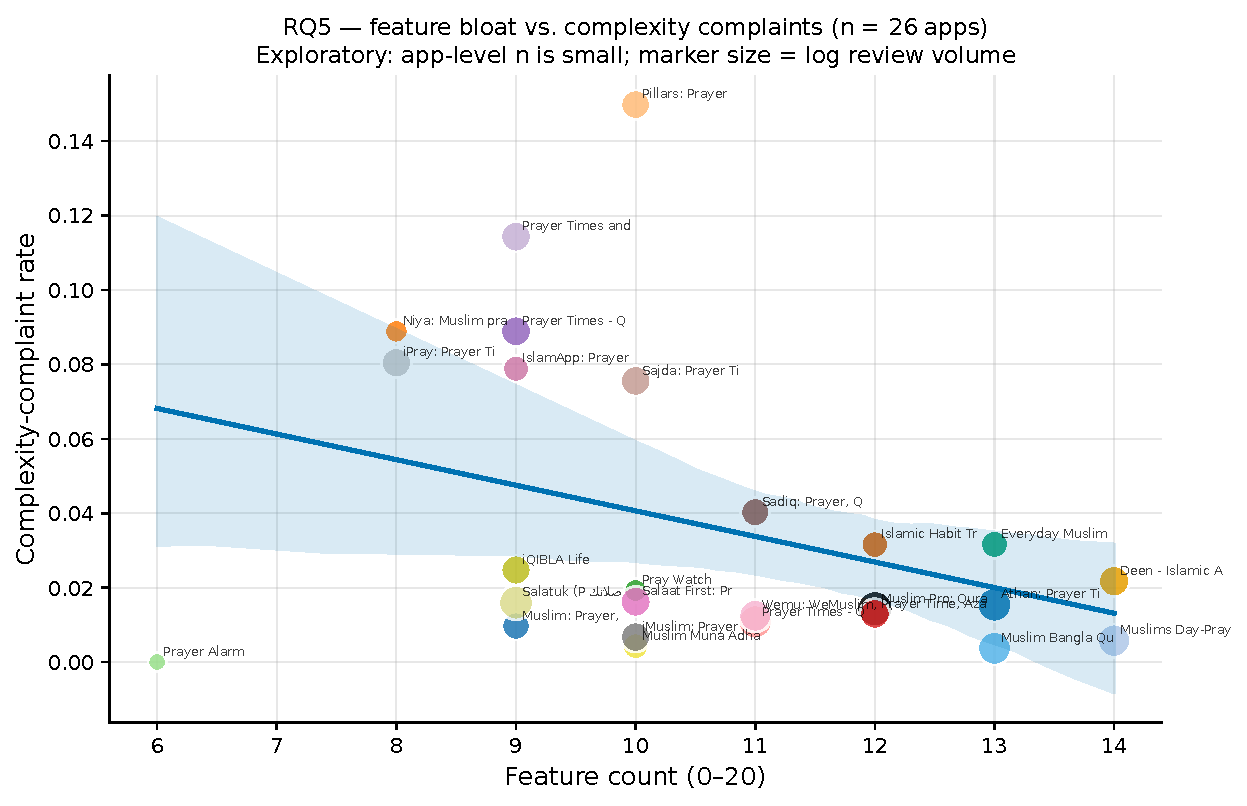
\includegraphics[width=\linewidth]{fig08_rq5_bloat_curve}
  \caption{Bloat-complaint rate against feature count. The leanest apps draw bloat complaints at more than three times the rate of the fullest.}
  \label{fig:rq5-bloat-curve}
\end{figure}

\subsection{Bloat Complaints Are Interface Complaints}

If feature count is not the driver, what is? A review complaining about bloat
is 23.98 times more likely than base rate to also complain about the interface
(Fisher exact OR \(= 29.41\), \(p = 7.4\times10^{-137}\), \(n = 324{,}687\)).
The informative cell is small, and we give it rather than let the corpus-wide
\(n\) stand in: 134 reviews carry both complaints, 94 fusing them into a single
phrase and 40 keeping them in separate sentences. Restricting to those 40, the
lift is still 7.62\(\times\) (OR \(= 8.78\), \(p = 9.3\times10^{-24}\)). The
two lexicons share no keyword and no regex pattern, so a fused sentence carries
two distinct terms rather than one phrase counted twice. We report
7.62\(\times\) as the conservative bound but foreground the fused cases, since
they are literally what users say: bloat is voiced \emph{as} a property of the
interface.

\begin{quote}
\itshape ``Widget takes up too much space, [5\texttimes{}2], but displays
information only in [4\texttimes{}1]. Remaining blocks are blank, unusable for
other apps, just hogging space. Otherwise, good app, used daily. Has more than
timetables which for me is just unimportant clutter.''
\end{quote}
\hspace*{1em}--- Athan: Prayer Times \& Al Quran, 4 stars

\subsubsection{Provenance}
\label{sec:rq5-provenance}

The co-occurrence hypothesis and its test were specified on 2026-08-26, before
the full corpus was run, and that pre-registration stands. The decision to
foreground the fused cases, rather than lead with the conservative
separate-sentence bound, was made afterward with the co-occurrence figures and
labelled sub-topics already visible. The hypothesis and test were
pre-specified; the choice of reporting emphasis was not.

\subsection{The Sub-Topic Model Agrees, from a Different Direction}

A topic model fitted on \texttt{complexity\_bloat} reviews alone corroborates
the interface framing independently. Its labelled topics are dominated by
simplicity as something users \emph{praise} --- \emph{app praised for
simplicity} recurs across three topics, alongside \emph{praise for minimalistic
UI} and \emph{app praised for having no ads} --- with clutter, advertising, and
slowness (\emph{ads cause confusion while using app}, \emph{complaint for app
being slow}) on the negative side. Users are evaluating how much the interface
puts in front of them, not how many features the app contains. Topic structure
here is seed-sensitive (6--11 topics across five fixed seeds, mean pairwise ARI
0.452), so we report recurring themes rather than a fixed partition.

\subsection{Companion Hardware: A Case Study, \(N = 1\)}

One application, iQIBLA Life, ships a companion hardware device; of the 25
without one, 23 mention companion hardware only to request it. Inside iQIBLA
Life, hardware-aspect sentiment is 37.7\% negative and 45.9\% positive (518
mentions); across the 23 apps without hardware, mentions run 49.2\% negative
and 20.8\% positive (1,994 mentions), largely unmet requests for watch or ring
support rather than complaints about a device that exists. Shipping companion
hardware is therefore associated with \emph{better} hardware-topic sentiment
--- the reverse of a bloat story, and consistent with \S\ref{sec:rq3}'s finding
that unmet requests read more positively than usage reports of a feature that
can fail. The \texttt{companion\_hardware} tagger runs at 40\% precision (95\%
CI [12, 77]), so of 2,512 tagged mentions roughly 1,005 are genuine (interval
[295, 1{,}932]). With one treated application this is a descriptive case study;
no between-app estimate is possible.

\begin{quote}
\itshape ``app is not user friendly. often face problems of ring connectivity
and staff handling the problems is very incompetent and highly
unprofessional''
\end{quote}
\hspace*{1em}--- iQIBLA Life, 1 star


% results_rq6

\section{RQ6: Completeness and the Two Gaps}
\label{sec:rq6}

The final research question asks whether current devotional apps are enough, in
the sense the ``apps under-serve niche needs'' framing implies. The answer is
no, but that word conceals two structurally different failures calling for
different remedies. A \emph{coverage gap} is a market failure: entire
categories of need are served by a minority of the ecosystem despite measurable
demand. A \emph{delivery gap} is a quality failure, and the more damning,
because it falls on promises apps have already made --- including the most
basic ones.

\subsection{RQ6a: The Delivery Gap}

We compared each application's store-description promises against the sentiment
its reviews record. Of 272 promised (application, feature) pairs, 136 carry
enough mentions to judge reliably (\(n \geq 30\)); of those, 18 are broken
promises across 11 applications --- a claimed feature drawing over 40\%
negative sentiment. Table~\ref{tab:rq6-broken} ranks the break rate by share of
promising applications and Figure~\ref{fig:rq6a-delivery-gap} shows the full
gap. The two largest by mention volume are both Muslim Pro's: reminders/adhan
(9,989 mentions, 45.6\% negative) and monetisation terms (9,182 mentions,
54.8\% negative).

\begin{table}[t]
  \centering
  \small
  \caption{Features with at least one broken promise among those with \(n \geq 30\) judgeable mentions and more than one promising application. \texttt{tracker\_score}, with a single promising application, is discussed below rather than listed.}
  \label{tab:rq6-broken}
  \begin{tabular}{lr}
    \toprule
    Feature & Broken / promising apps \\
    \midrule
    Monetisation             & 5 / 16 (31\%) \\
    Reminders / adhan        & 5 / 20 (25\%) \\
    Mosque finder             & 1 / 4 (25\%) \\
    Forbidden times            & 1 / 4 (25\%) \\
    Widgets                    & 2 / 13 (15\%) \\
    Prayer-time accuracy      & 2 / 19 (11\%) \\
    Qibla                      & 1 / 18 (6\%) \\
    \bottomrule
  \end{tabular}
\end{table}

Two rows carry a caveat: forbidden times is tagged at 10\% precision and mosque
finder at 27\% (\S\ref{sec:method-measurement}), so their 1-of-4 ratios rest on
few and noisy mentions, and we rest no argument on either.

\begin{figure}[t]
  \centering
  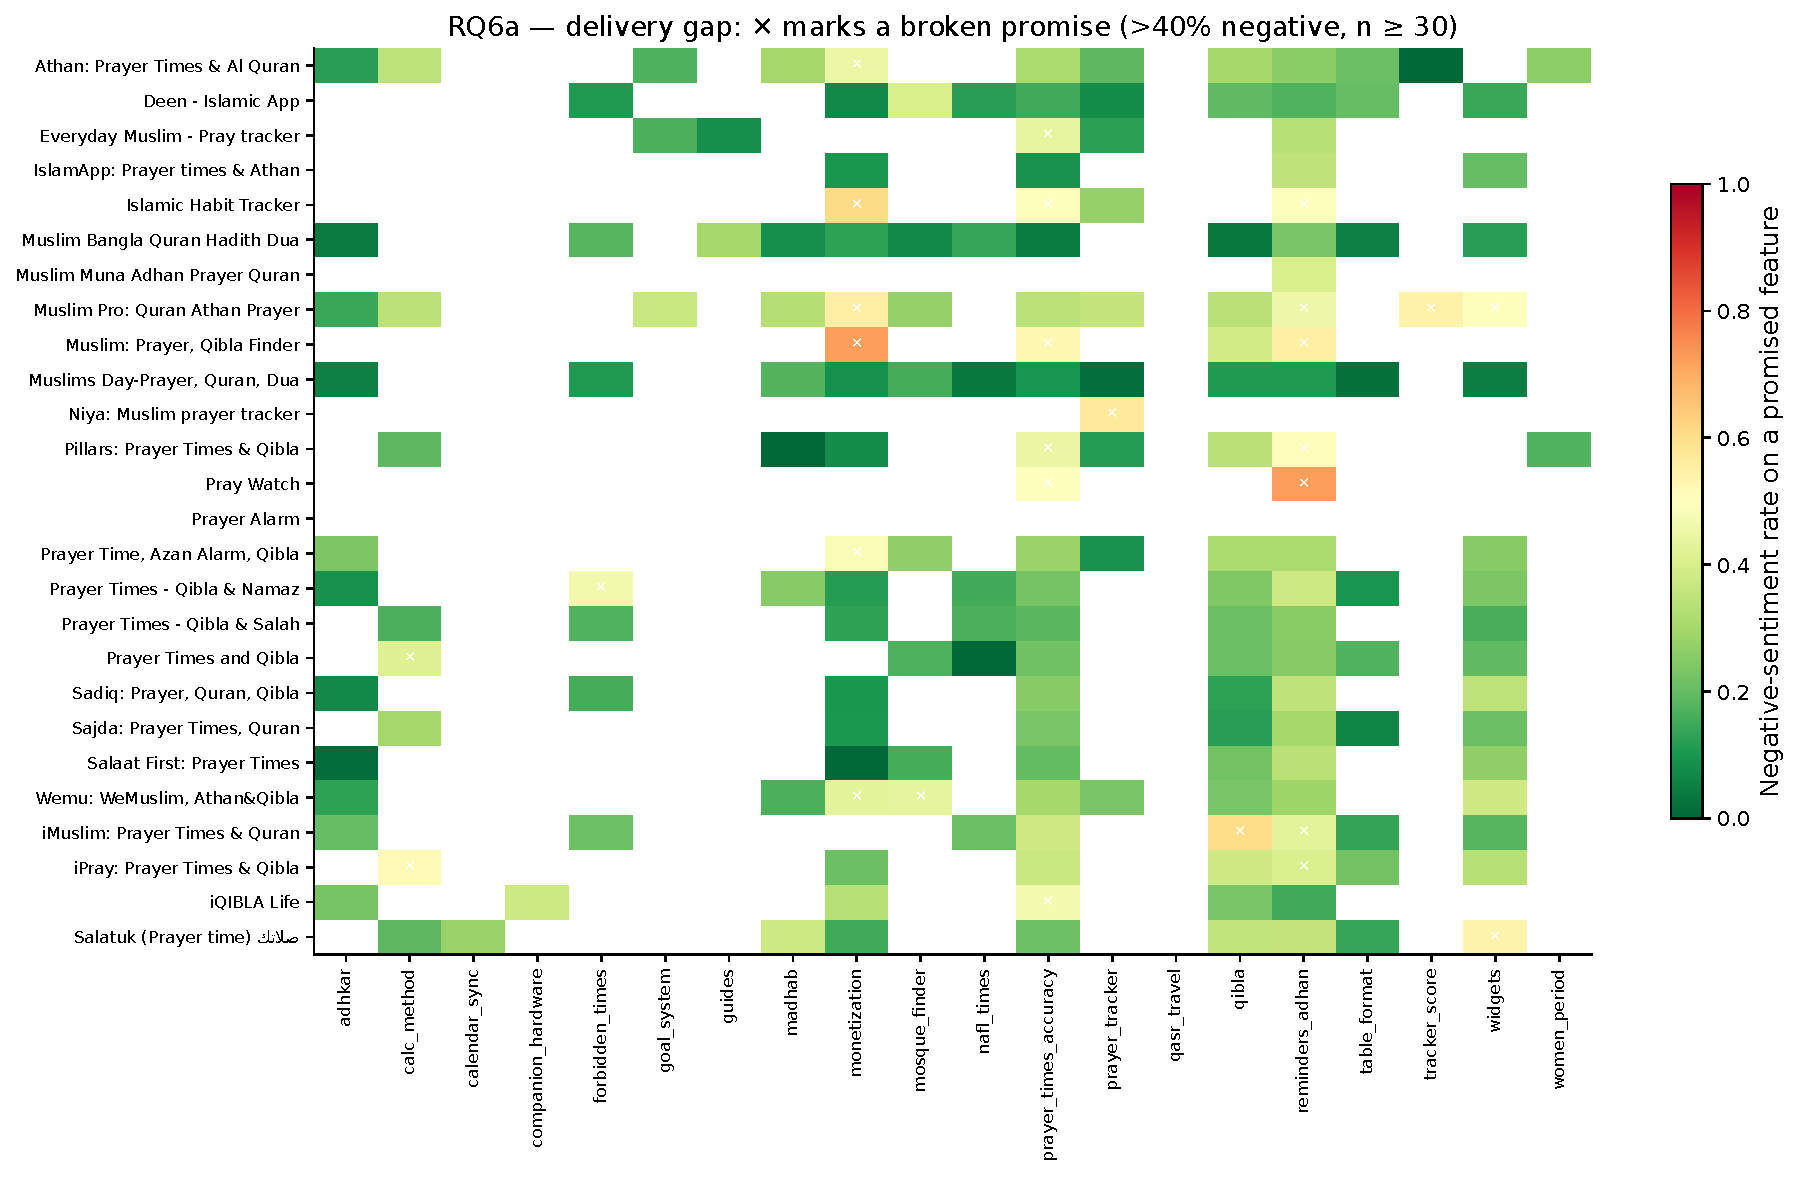
\includegraphics[width=\linewidth]{fig10_rq6a_delivery_gap}
  \caption{The delivery gap: negative-sentiment rate per (application, feature) pair across the 136 judgeable pairs.}
  \label{fig:rq6a-delivery-gap}
\end{figure}

One further aspect, \texttt{tracker\_score}, shows 1 of 1 promising
applications broken; with a single promising application the ratio carries no
statistical weight, so we do not present it as the most-broken feature.

The two features broken in the most applications, five each, are also the two
most basic. Adhan reminders are the core function of a prayer-times
application, and monetisation the terms on which it is offered. Failure here
concentrates in the promise the app is built around, not in peripheral
functionality.

\subsection{RQ6b: The Coverage Gap}

We separately ranked aspects by an unmet-need score --- demand-signal volume
multiplied by applications lacking the feature --- built from the
demand-extraction pipeline validated at 91.5\% precision
(\S\ref{sec:method-demand}) rather than from the noisier raw aspect counts
several low-precision aspects would otherwise force on us
(Table~\ref{tab:rq6-unmet}, Figure~\ref{fig:rq6b-unmet-needs}). Companion
hardware tops the ranking, followed by menstrual handling, mosque finder,
forbidden-times awareness, and \emph{nafl} (supererogatory) prayer-time
support. Four aspects fall below 25\% ecosystem coverage:
\texttt{calendar\_sync}, \texttt{companion\_hardware}, \texttt{qasr\_travel},
and \texttt{women\_period}.

\begin{table}[t]
  \centering
  \small
  \caption{Unmet-need ranking: demand-signal volume \(\times\) applications lacking the feature.}
  \label{tab:rq6-unmet}
  \begin{tabular}{lrr}
    \toprule
    Aspect & Score & Apps lacking \\
    \midrule
    Companion hardware & 6{,}725 & 25 \\
    Menstrual handling (\texttt{women\_period}) & 4{,}738 & 23 \\
    Mosque finder       & 3{,}304 & 14 \\
    Forbidden times      & 2{,}805 & 15 \\
    Nafl (supererogatory) prayer times & 2{,}445 & 15 \\
    \bottomrule
  \end{tabular}
\end{table}

\begin{figure}[t]
  \centering
  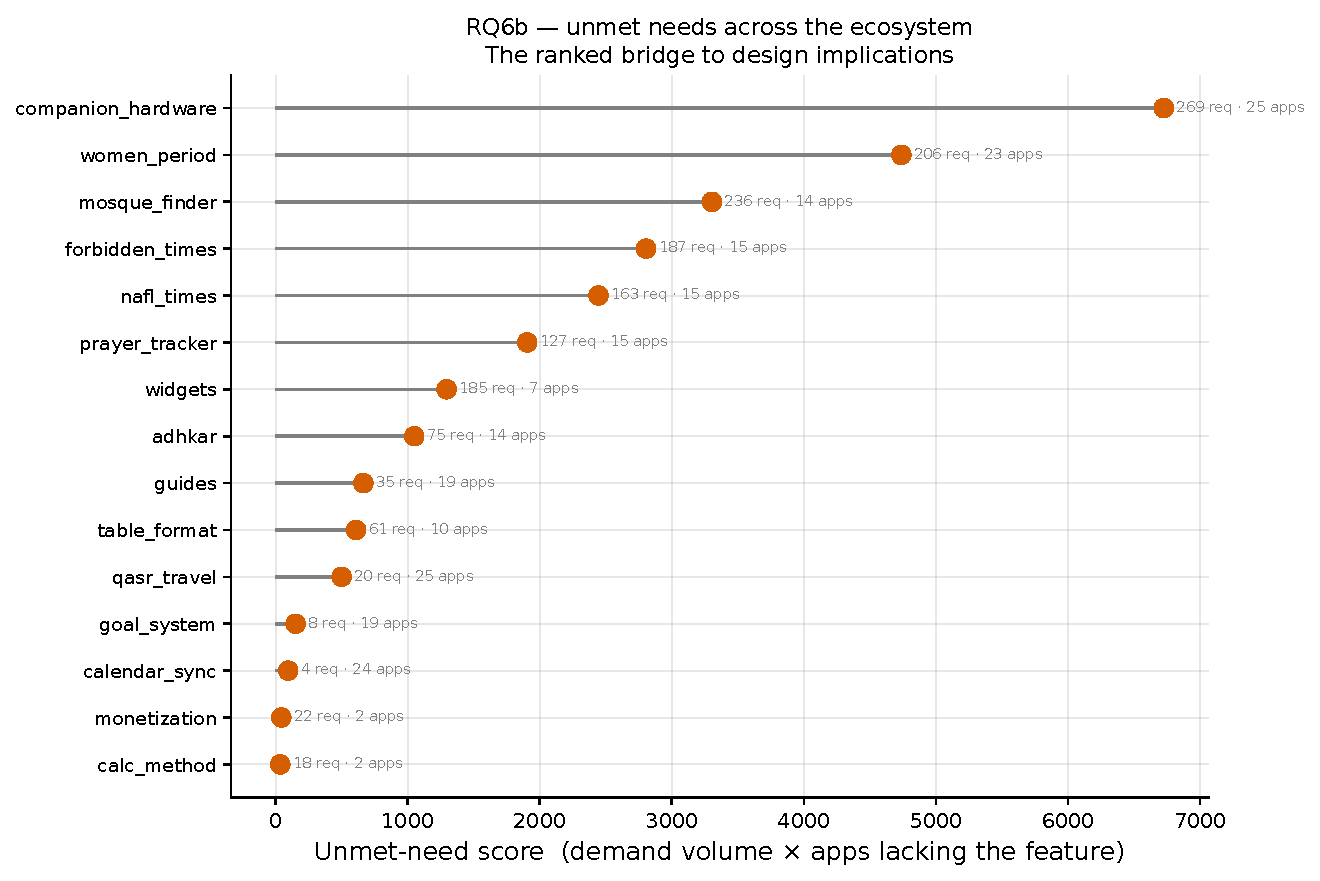
\includegraphics[width=\linewidth]{fig11_rq6b_unmet_needs}
  \caption{Unmet-need ranking across aspects: demand-signal volume against the number of applications lacking the feature.}
  \label{fig:rq6b-unmet-needs}
\end{figure}

\subsection{Some Needs Are Served Well}

Five aspects clear both bars we set for adequate service --- present in over
half the ecosystem, averaging under 30\% negative sentiment across the
applications where mentioned: madhab, monetisation, qibla, table format,
widgets. Table format is tagged at 44\% precision, so its place is the least
secure. The average is taken over applications rather than reviews, which
matters: under review-weighted pooling, monetisation, widgets, and qibla all
exceed 30\%, because a few high-volume applications handle them badly. We
report the app-level figure because the question is how many applications serve
a need adequately, not how many reviews are unhappy, but the choice should not
pass unnoticed.

Monetisation appears on both this list and the broken-promises list in
Table~\ref{tab:rq6-broken}, which is informative rather than contradictory.
Across the same 16 applications promising it with \(n \geq 30\) mentions, the
break rate is 5 of 16 (31\%) against a mean negative rate of 25.8\%: most
handle payment acceptably while a minority handle it badly enough to poison the
feature ecosystem-wide.

\subsection{Synthesis: The Same Gaps, Reached Independently}

Both gaps are also reached independently by an earlier research question, which
we read as corroboration rather than repetition. Companion hardware tops the
unmet-need ranking, and RQ5 finds hardware sentiment \emph{better} inside the
one application shipping a device than across the 23 that do not
(\S\ref{sec:rq5}) --- demand rather than dissatisfaction with an existing
product. Menstrual handling ranks second and is RQ4's central finding in its
own right (\S\ref{sec:rq4}). Reminders/adhan, tied with monetisation at five
broken applications each, is independently the dominant
tracker-dissatisfaction theme in RQ1's cross-app coding (\S\ref{sec:rq1}).

\subsection{Verdict}

Current applications are not enough, and fall short in two ways calling for
different responses. The coverage gap is a market failure: entire categories of
need --- companion hardware, menstrual accommodation, travel concession,
calendar integration --- are served by under a quarter of the ecosystem despite
measurable, explicitly voiced demand. The delivery gap is a quality failure and
the more damning, because it falls on promises already made: the features most
often broken are adhan reminders and monetisation, the two things a
prayer-times application most fundamentally offers. Building more features is
not indicated. Delivering the promised ones reliably, and extending coverage to
the populations currently unserved, is.

% results_discussion

\section{Discussion}
\label{sec:discussion}

Across six research questions, one pattern recurs: satisfaction with a
devotional app is governed by the reliability of its core functions, not by
how many features it offers, and three framings borrowed from the broader HCI
and self-tracking literatures mis-locate where the problem sits. We take up
what each reframing changes, then what the paper implies methodologically for
research on app-store reviews beyond this domain. The prescriptive
consequences are collected separately in \S\ref{sec:design-implications}.

\subsection{Three Reframings}

\textbf{Gamification.} The harm the self-tracking literature predicts is guilt
induced by streaks and scores. That is not what we find (\S\ref{sec:rq1}). The
harm is a record users cannot trust and a prompt that does not arrive: an app
that loses logged history, regresses a count, or silently stops prompting
before logging is even at issue. Where a genuinely normative objection does
surface, it is not that the app makes the user feel judged; it is that the app
\emph{models worship incorrectly} --- no menstrual exemption, no support for
supererogatory (\emph{sunnah}) prayer, imposed goals that displace a user's own
targets. Softening a streak mechanic does not address a tracker that does not
know a user is exempt from prayer that day.

\textbf{Accuracy versus aesthetics.} The trade-off this framing poses is
mis-specified (\S\ref{sec:rq2}). Accuracy is not one thing to be weighed
against interface polish: prayer-time correctness behaves like a reliability
requirement, disjoint in cost from every interface complaint and carrying the
corpus's second-highest penalty, while madhab configuration behaves like an
ordinary preference, cheap to get wrong and reversing sign under a robustness
check. Treating ``accuracy'' as a single design dimension obscures exactly the
distinction that matters for prioritisation.

\textbf{Feature bloat.} What users call bloat is a property of what the
interface \emph{surfaces} in the moment, not of how many capabilities the
application \emph{contains} (\S\ref{sec:rq5}). The feature-count framing cannot
express that distinction, which is why it fails in both directions at once: no
relationship to bloat complaints where one is predicted, and an inverse one
where none is.

\subsection{The Two Gaps}

RQ6 (\S\ref{sec:rq6}) names two failures that the other five research questions
independently arrive at from different directions. Coverage is a \emph{market
failure}: whole categories of need are served by under a quarter of the
ecosystem despite demand that is explicit and easy to find in review text.
Delivery is a \emph{quality failure}, and the more consequential, because it
falls on promises applications have already made rather than on capabilities
they never claimed. The two most-broken promises in the corpus are adhan
reminders and monetisation terms, which is to say the core function of a
prayer-times app and the terms it is offered on.

\subsection{Methods Implications}

Two of this paper's four contributions are methodological, and they carry three
lessons for app-store review research beyond this domain.

\textbf{Star ratings are an unsafe proxy for defect severity.} 41.6\% of
reviews carrying a negative accuracy complaint award four or five stars
(\S\ref{sec:rq2}). A defect-prioritisation process that reads severity off the
star distribution --- the signal most app-store ranking and triage systems are
built around --- will systematically under-weight exactly the class of defect
users are least willing to let tank their rating. Text, not stars, is where
this class of complaint is visible.

\textbf{Single-app qualitative sampling can manufacture genre-level themes.}
Themes that looked like general properties of gamified prayer tracking
accounted for 51\% of a single-application coding pass and only 4\% of an
independently drawn, stratified cross-application pass on the same phenomenon
(\S\ref{sec:rq1-coding}). Both samples were coded in good faith; the difference
is entirely in what a selection rule's tie-break happened to return. Any
qualitative app-review study drawing its sample from one application, even
inadvertently, should treat its themes as a hypothesis about that application
until checked against others.

\textbf{Devotional register breaks off-the-shelf NLP.} A feature-vocabulary
match scored 0\% precision on its own gold rows because reviewers routinely
close devotional app reviews with formulae such as ``May Allah reward you,''
which generic goal-related keywords mistake for feedback about a tracking
feature (\S\ref{sec:method-devotional-filtering}). Anyone applying
general-purpose sentiment or aspect tooling to religious or otherwise
register-heavy text should expect this failure and budget for a filtering pass
before trusting aspect-level output.

\subsection{Three Threads}

Three concerns recur across research questions rather than belonging to any
one, and naming them is part of what makes six research questions a single
argument. \emph{Advertising and monetisation} run together through the results without
being the same thing: intrusive advertising is the costliest complaint in the
corpus by coefficient (\S\ref{sec:rq2}) and a dominant theme in bloat discourse
(\S\ref{sec:rq5}), while monetisation, tracked separately in our lexicon, is an
RQ1 coding theme and one of RQ6's two most-broken promises. \emph{Adhan reminders} are the most-cited reason users give for
choosing an app (\S\ref{sec:rq3}), one of the two most-broken promises
(\S\ref{sec:rq6}), and the dominant tracker-dissatisfaction theme at 46\%
(\S\ref{sec:rq1}). Beneath both sits a concern with \emph{the record rather
than the streak}: RQ1's reframing of gamification harm, RQ4's menstrual
exemption as a record the app gets wrong rather than a feature it lacks, and
RQ6's coverage gap are three instances of one underlying want --- an accurate,
owned, accommodating record of one's own worship.

% results_limitations

\section{Limitations}
\label{sec:limitations}

We state these plainly rather than as hedges: each has a claim ceiling the
results above already respect.

\begin{itemize}

\item \textbf{No users were studied.} Every finding is inferred from public
app-store reviews, a self-selected sample skewed toward strong positive and
strong negative experiences and at best an indirect proxy for lived religious
practice. Claims about user experience here are claims about what reviewers
chose to write down.

\item \textbf{The corpus is an English/US-locale slice, and the applications
were chosen purposively} (\S\ref{sec:method-corpus}), so it under-represents
the regions where most of the world's Muslims live. The aspects most exposed
are the regionally patterned ones --- madhab, calculation method, travel
concession --- so RQ2's finding that madhab complaints are mild and cheap is
not a global claim. Because every application was collected under identical
parameters, this limits generalisation rather than threatening the comparisons
between them.

\item \textbf{Aspect-tagging precision is uneven.} Seven of the 25 aspects with
surviving gold rows fall below 50\%, two at 0\%
(\S\ref{sec:method-measurement}); counts for those seven are paired with
precision-adjusted estimates. The five models draw on aspects at 64--100\%
precision with two exceptions flagged at the point of use. Noise of this kind
attenuates effects toward zero rather than manufacturing them, so it works
against the paper's claims.

\item \textbf{Eleven model terms cannot support inference.} Eight are
non-converged rather than precisely estimated nulls, retained in the
Benjamini--Hochberg denominator of 29, where they are eight of the nine terms
failing correction; the other three return neither a standard error nor a
\(p\)-value and sit outside it (\S\ref{sec:method-models}). Every null reported
here is cited from a fit that converged.

\item \textbf{The topic model characterises a minority of the corpus, and its
structure is seed-sensitive.} 22.7\% of modelled documents fall in the outlier
bucket and 61\% in a single undifferentiated praise cluster; the 39 topics we
label cover about 16\%. The \texttt{rq5\_bloat} sub-model yields 6 to 11 topics
across five fixed seeds (mean pairwise ARI 0.452), so we claim the recurring
themes such a model surfaces, not a specific partition.

\item \textbf{The RQ4 sub-model collapsed around one application's privacy
episode.} Six of ten topics sit on a single theme concerning one application's
user data being sold to US military-linked buyers, holding 58\% of the
sub-model's non-outlier documents. That application is Muslim Pro, whose
November 2020 data-sale reporting we name explicitly because the finding is
specific to that episode rather than a property of the ecosystem; it precludes
further resolution of menstrual-handling discourse (\S\ref{sec:rq4}).

\item \textbf{Illustrative quotations skew toward one application.} Seven of
the 13 reviews quoted come from Athan, the corpus's largest tracker-bearing
application, because quotation followed the volume of available text rather
than a sampling rule --- the same hazard we identify as a methodological
contribution (\S\ref{sec:rq1-coding}). Every claim they illustrate rests on the
corpus-scale or cross-application evidence reported alongside them.

\item \textbf{The affect lexicon is unvalidated.} The guilt and motivation
keyword lists behind RQ1's lexical comparison have no gold sample and no
precision figure, and their vocabulary overlaps ordinary praise and defect
language (\S\ref{sec:method-affect}). RQ1's claim about guilt rests on the
hand-coded passes, which point the same way.

\item \textbf{Two qualitative coding passes, never pooled} (\S\ref{sec:rq1-coding}),
coding 80 reviews between them. They are supporting evidence that sharpens the
corpus-scale results, not a primary contribution.

\item \textbf{Three small-\(N\) case studies are descriptive only.} Inclusion
features ship in 3 of 26 applications; companion hardware and qasr travel
concession each in exactly 1. None supports a between-app statistical estimate,
and we report none.

\item \textbf{Promise-source agreement is weak.} Store descriptions and the
hand-built feature matrix agree at a mean Cohen's \(\kappa\) of 0.272, against
73.1\% mean raw agreement, with four features at \(\kappa = 0\) as a prevalence
artefact (\S\ref{sec:method-promise}). Any claim depending on what an
application promises carries that ceiling.

\item \textbf{The demand-precision sample predates the final extraction.} The
200-row gold sample behind the 91.5\% figure was labelled against an earlier
run; current demand counts come from the regenerated extraction
(\S\ref{sec:method-demand}).

\item \textbf{Topic modelling covers English-identified text only.} Of 324,687
texted reviews, fastText identified 276,422 as English, and only that subset
entered topic modelling, so topic-model findings do not characterise discourse
in the excluded languages.

\item \textbf{Reviews are cross-sectional, not longitudinal.} Nothing links a
user's reviews across time, so we can speak to aggregate patterns but not to
how an individual's relationship with an application changes over their tenure.

\end{itemize}

% results_design_implications

\section{Design Implications}
\label{sec:design-implications}

We do not recommend adding features generically: feature count is not the
lever satisfaction runs on. Each recommendation ties to a specific reported
result, and every coverage recommendation pairs with its delivery point, since
the two gaps need different remedies.

\subsection{Deliver What Is Already Promised, Before Adding Anything}

The two most-broken promises are also the two most basic: adhan reminders
(broken in 5 of 20 promising applications) and monetisation terms (5 of 16)
(\S\ref{sec:rq6}). Prompting failure is independently the dominant tracker
complaint, at 46\% of the cross-app coding pass (\S\ref{sec:rq1}). An
application that cannot reliably fire a notification cannot support a
prayer-tracking practice built on top of it, whatever else it ships.

\subsection{Treat Prayer-Time Correctness as a Reliability Requirement}

Prayer-time accuracy costs \(-1.112\) stars, the second-costliest of the
complaint aspects we model, and 41.6\% of accuracy complaints arrive inside
four- or five-star reviews (\S\ref{sec:rq2}). A team prioritising defects from
its own rating distribution will systematically under-prioritise this class of
failure. We recommend instrumenting for accuracy defects directly, comparing
computed times against an authoritative reference, rather than inferring
severity from ratings that conceal them.

\subsection{Accommodate Practice, Rather Than Softening Mechanics}
\label{sec:design-accommodate}

Where tracker dissatisfaction carries a normative complaint, it is that the
app mis-models worship, not that its mechanics apply too much pressure
(\S\ref{sec:rq1}). Menstrual handling makes this concrete: it ranks second on
the unmet-need index, is absent from 23 of 26 applications, and in the three
that do ship it, sentiment is no better than in applications without it
(\S\ref{sec:rq4}). This is simultaneously a coverage problem and a quality
problem; closing the coverage gap without fixing reliability would not resolve
it.

\subsection{Surface Less; Do Not Necessarily Contain Less}

The lever available to a design team is what the interface surfaces in a
given moment, not how many capabilities the application contains
(\S\ref{sec:rq5}). A full-featured application with a disciplined interface is
not the problem the bloat framing warns against; a lean application that
surfaces its few features poorly can still earn the complaint.

\subsection{The Unserved Categories}

Four categories fall below a quarter of ecosystem coverage against
demonstrated demand (\S\ref{sec:rq6}). \textbf{Companion hardware} tops the
ranking, absent from 25 of 26 applications, and sentiment toward hardware is
\emph{better} inside the one application shipping a device (\S\ref{sec:rq5}),
so this is demand rather than dissatisfaction with an existing product.
\textbf{Menstrual accommodation} ranks second (\S\ref{sec:design-accommodate}).
\textbf{Travel concession} (\emph{qasr}) has essentially no market presence
(\S\ref{sec:rq3}), and \textbf{calendar integration} rounds out the four.
None of these calls for adding features indiscriminately; each is a
demand-evidenced gap in an ecosystem whose more pressing problem is delivering
what it has already promised.



\bibliographystyle{ACM-Reference-Format}
\bibliography{references}

%%
%% End of file `sigconf.tex'.
\end{document}
